\setcounter{page}{1}
\setcounter{figure}{0}  % reset counter

\section{Supplemental results for the Yeast dataset}
\subsection{Results on unique MS3 -18 identifications}
\subsubsection{S,T, and Y are valid sites}

\begin{figure}[htbp]
\centering % trim=l b r t
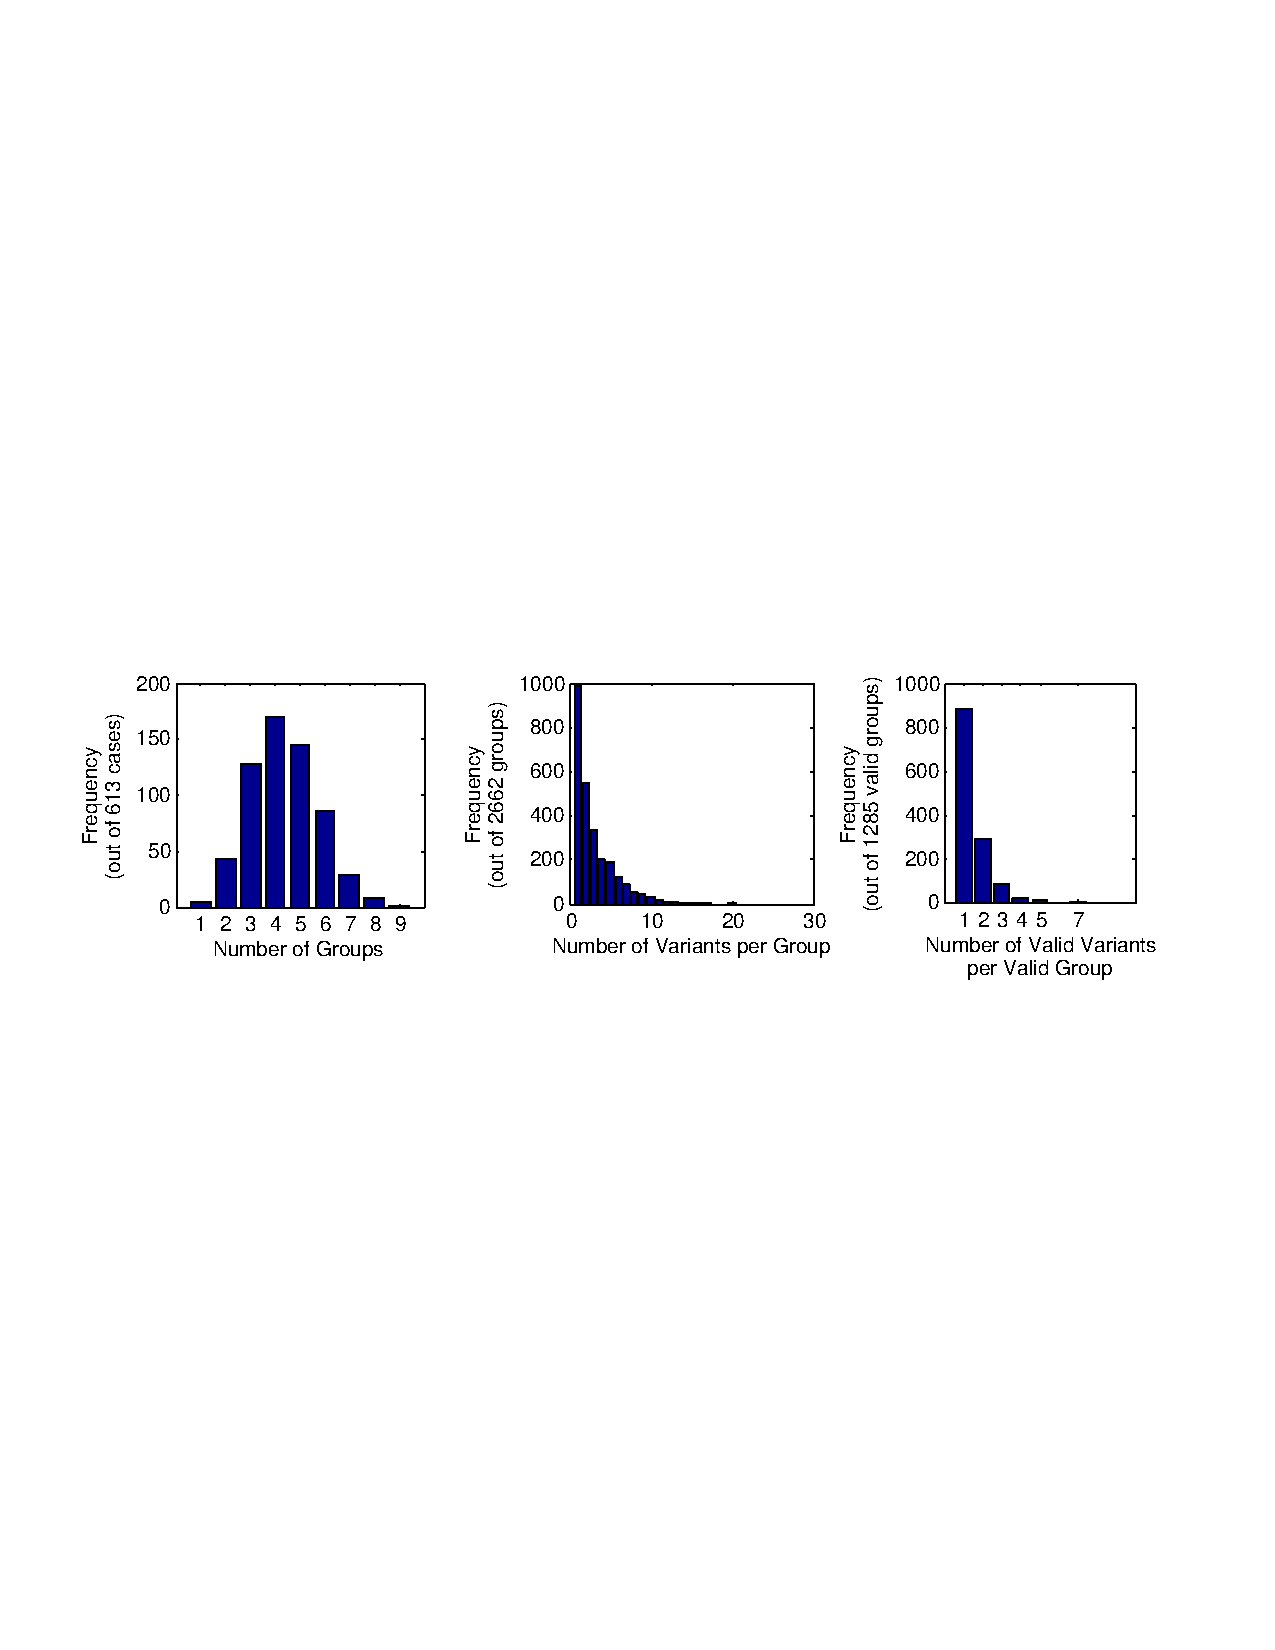
\includegraphics[trim = 2mm 105mm 4mm 105mm,
clip,width=\textwidth]{fig/phospho/uniqueIds/size_dist_uniq_by_STY.pdf}
\caption{Distribution of number of variant groups, size of variant groups, and number of valid variants per valid group.}
\label{fig:yeast_sizedist_STY}
\end{figure}


\begin{table}[h]
  \centering
  \caption{Yeast MS3 dataset PTM site assignment FLR results on unique peptide identifications. At cosine score cutoff = $0.4$, $52$ cases rejected, $561$ cases accepted. S, T and Y are considered as valid sites.}\label{tbl:YeastFLR_uniq_STY}
\begin{tabular}{|c|l|l|l|l|l|}
\hline
Estimated Abundance & \multirow{2}{*}{FDR} & \multicolumn{4}{|c|}{\#Cases with k groups identified }\\
of Variant Group & & $k\ge 1$ & $k=1$ & $k=2$ & $k=3$\\
\hline
$\ge	60	\%$ &	0.02	\% &	91.8	\% &	91.8	\% &	0.0	\% &	0.0	\\
$\ge	55	\%$ &	0.02	\% &	94.1	\% &	94.1	\% &	0.0	\% &	0.0	\\
$\ge	50	\%$ &	0.03	\% &	95.1	\% &	94.9	\% &	0.2	\% &	0.0	\\
$\ge	45	\%$ &	0.03	\% &	96.2	\% &	95.6	\% &	0.6	\% &	0.0	\\
$\ge	40	\%$ &	0.03	\% &	96.8	\% &	94.9	\% &	1.9	\% &	0.0	\\
$\ge	35	\%$ &	0.04	\% &	97.9	\% &	95.1	\% &	2.8	\% &	0.0	\\
$\ge	34	\%$ &	0.04	\% &	97.9	\% &	94.9	\% &	3.0	\% &	0.0	\\
$\ge	33	\%$ &	0.04	\% &	98.3	\% &	94.9	\% &	3.4	\% &	0.0	\\
$\ge	32	\%$ &	0.05	\% &	98.3	\% &	94.9	\% &	3.4	\% &	0.0	\\
$\ge	31	\%$ &	0.05	\% &	98.3	\% &	94.7	\% &	3.6	\% &	0.0	\\
$\ge	30	\%$ &	0.05	\% &	98.5	\% &	94.7	\% &	3.8	\% &	0.0	\\
$\ge	25	\%$ &	0.06	\% &	98.9	\% &	93.7	\% &	4.9	\% &	0.2	\\
$\ge	20	\%$ &	0.08	\% &	99.1	\% &	92.8	\% &	6.1	\% &	0.2	\\
%$\ge	15	\%$ &	0.11	\% &	99.4	\% &	91.8	\% &	7.4	\% &	0.2	\\
%$\ge	10	\%$ &	0.16	\% &	99.6	\% &	90.1	\% &	8.9	\% &	0.6	\\
%$\ge	5	\%$ &	0.23	\% &	99.8	\% &	84.6	\% &	14.4	\% &	0.8	\\
\hline
\end{tabular}
\end{table}

\begin{figure}[htbp]
\centering % trim=l b r t
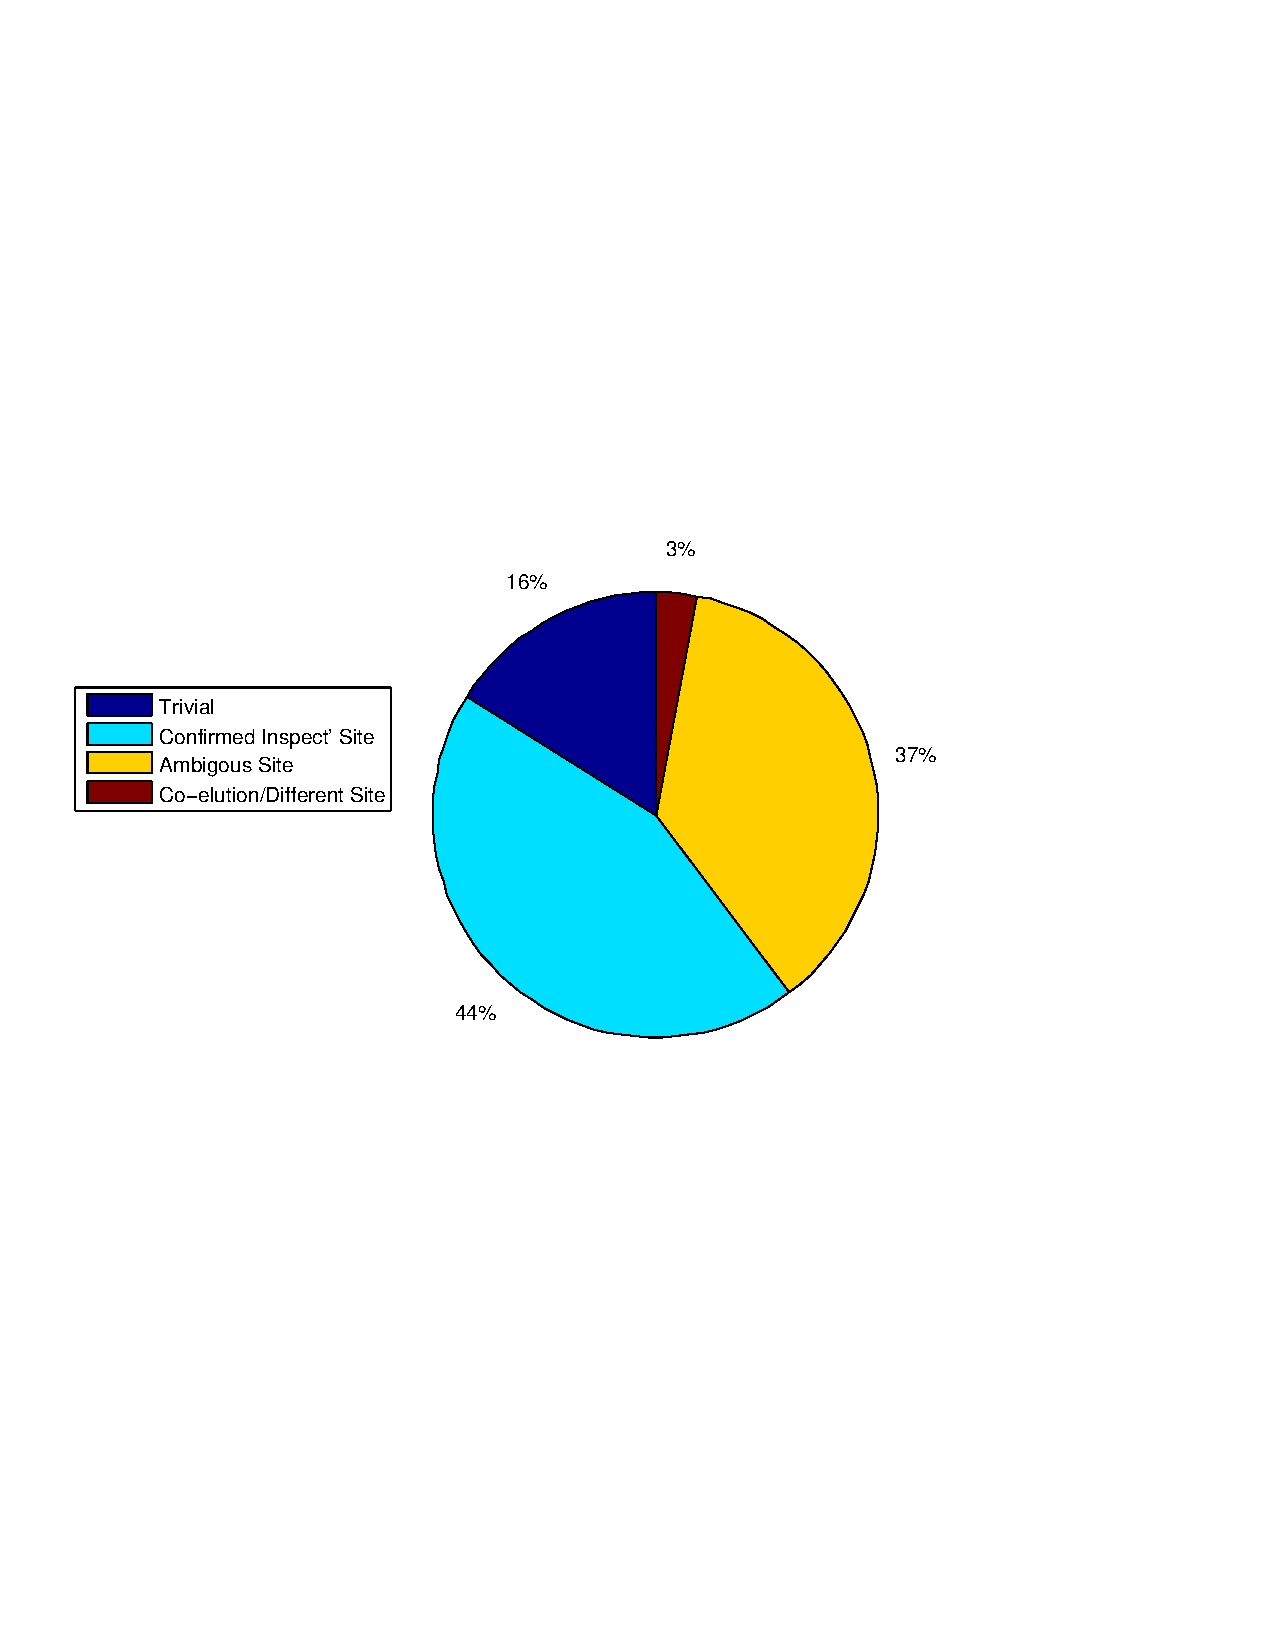
\includegraphics[trim = 0mm 90mm 20mm 90mm,clip,width=0.6\textwidth]{fig/phospho/uniqueIds/piechart_uniq_by_STY.pdf}
\caption{Yeast dataset results on unique MS3 -18 peptide identifications: Site assignment results for yeast dataset at $3\%$ FDR.}
\label{fig:yeast_piechart_uniqIds_STY}
\end{figure}

\clearpage
\subsubsection{S,T,Y,D, and E are valid sites}
\begin{figure}[htbp]
\centering % trim=l b r t
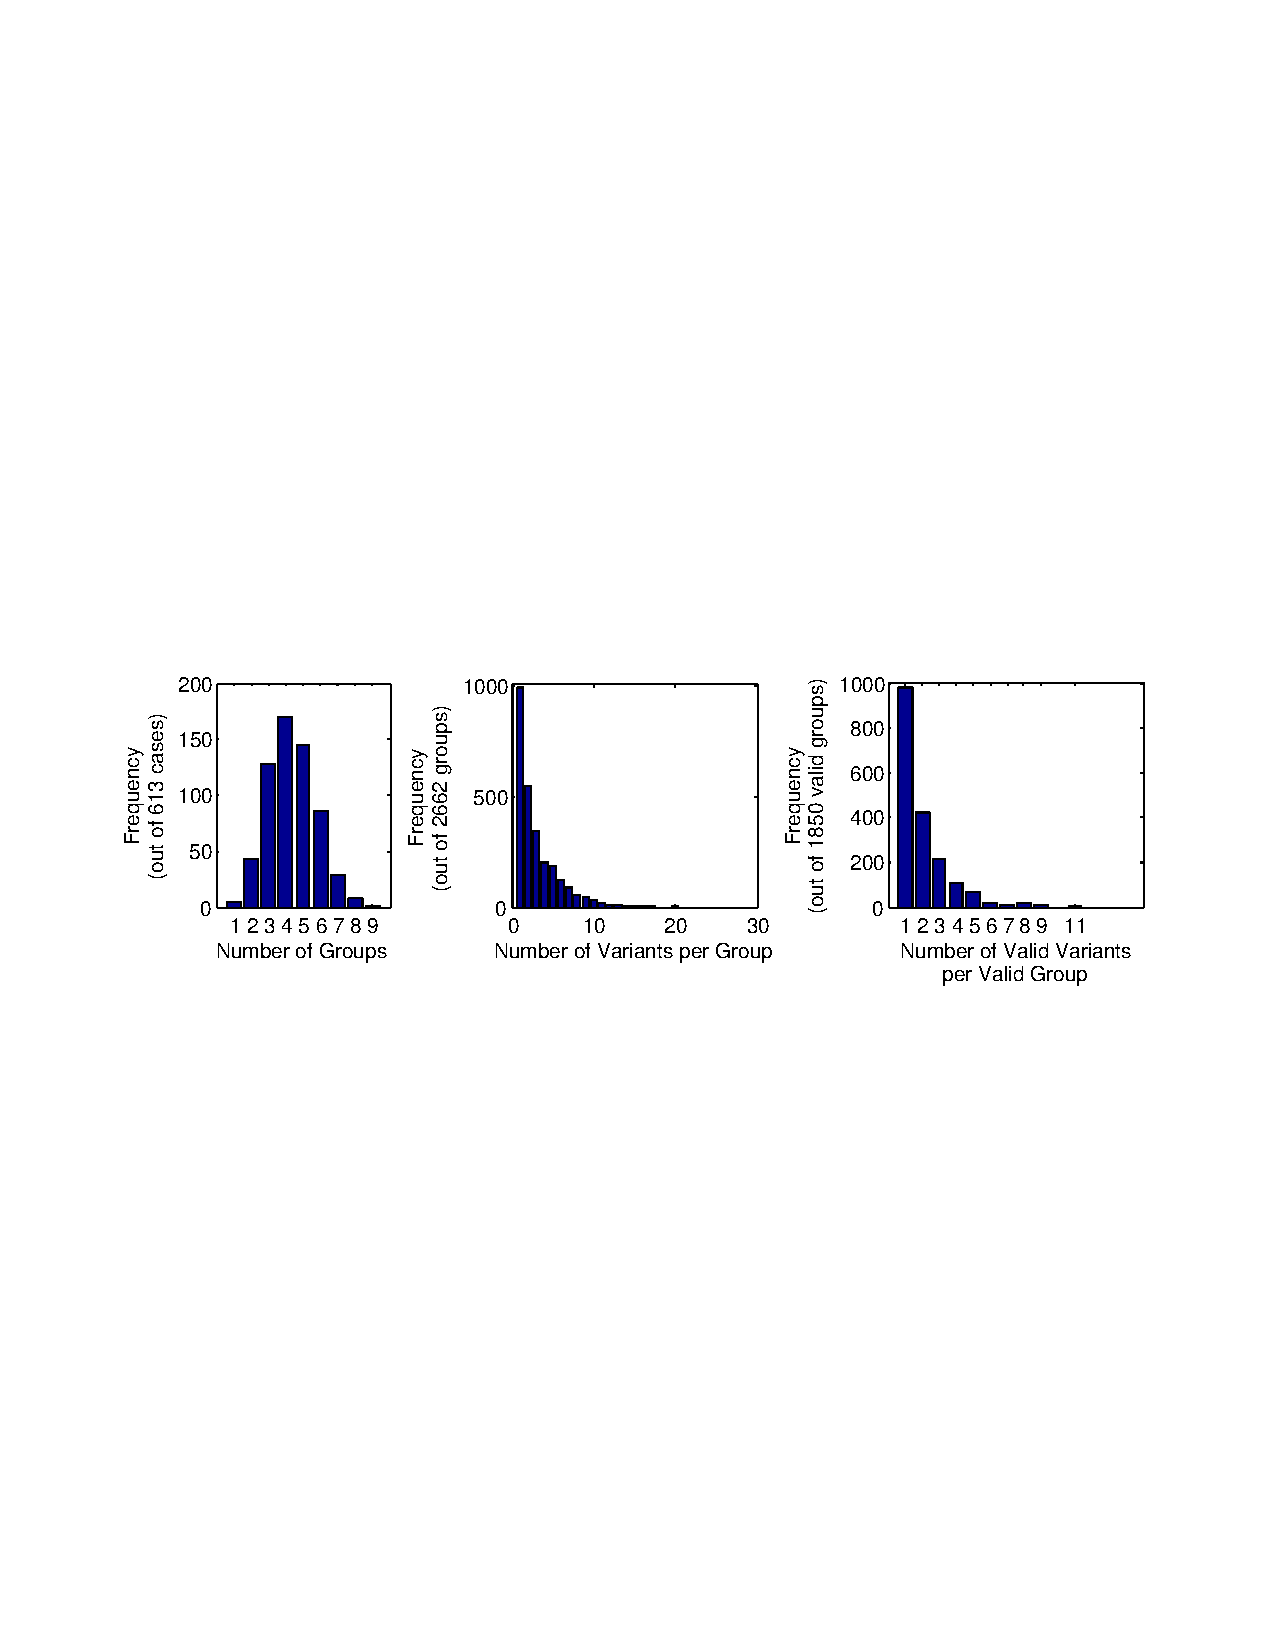
\includegraphics[trim = 2mm 105mm 4mm 105mm,
clip,width=\textwidth]{fig/phospho/uniqueIds/size_dist_uniq_by_STYDE.pdf}
\caption{Distribution of number of variant groups, size of variant groups, and number of valid variants per valid group.}
\label{fig:yeast_sizedist_STYDE}
\end{figure}

\begin{table}[h]
  \centering
  \caption{Yeast MS3 dataset PTM site assignment FLR results on unique peptide identifications. At cosine score cutoff = $0.4$, $52$ cases rejected, $561$ cases accepted. S, T, Y, D and E are considered as valid sites.}\label{tbl:YeastFLR_uniq_STYDE}
\begin{tabular}{|c|l|l|l|l|l|l|}
\hline
Estimated Abundance & \multirow{2}{*}{FDR} & \multicolumn{5}{|c|}{\#Cases with k groups identified }\\
of Variant Group & & $k\ge 1$ & $k=1$ & $k=2$ & $k=3$  & $k=4$\\
\hline
$\ge	60	\%$ &	0.01	\% &	90.6	\% &	90.6	\% &	0.0	\% &	0.0	\% &	0.0	\\
$\ge	55	\%$ &	0.02	\% &	92.7	\% &	92.7	\% &	0.0	\% &	0.0	\% &	0.0	\\
$\ge	50	\%$ &	0.02	\% &	93.6	\% &	93.4	\% &	0.2	\% &	0.0	\% &	0.0	\\
$\ge	45	\%$ &	0.02	\% &	94.3	\% &	93.8	\% &	0.5	\% &	0.0	\% &	0.0	\\
$\ge	40	\%$ &	0.02	\% &	94.8	\% &	92.7	\% &	2.1	\% &	0.0	\% &	0.0	\\
$\ge	35	\%$ &	0.03	\% &	95.7	\% &	92.3	\% &	3.4	\% &	0.0	\% &	0.0	\\
$\ge	30	\%$ &	0.03	\% &	96.4	\% &	91.6	\% &	4.8	\% &	0.0	\% &	0.0	\\
$\ge	25	\%$ &	0.04	\% &	96.6	\% &	89.7	\% &	6.8	\% &	0.2	\% &	0.0	\\
$\ge	20	\%$ &	0.05	\% &	96.6	\% &	86.8	\% &	9.4	\% &	0.4	\% &	0.0	\\
%$\ge	15	\%$ &	0.05	\% &	97.0	\% &	84.1	\% &	11.8	\% &	1.1	\% &	0.0	\\
%$\ge	10	\%$ &	0.06	\% &	97.0	\% &	78.3	\% &	16.8	\% &	1.6	\% &	0.4	\\
%$\ge	5	\%$ &	0.10	\% &	97.1	\% &	71.1	\% &	22.1	\% &	3.4	\% &	0.5	\\
\hline
\end{tabular}
\end{table}

\begin{figure}[htbp]
\centering % trim=l b r t
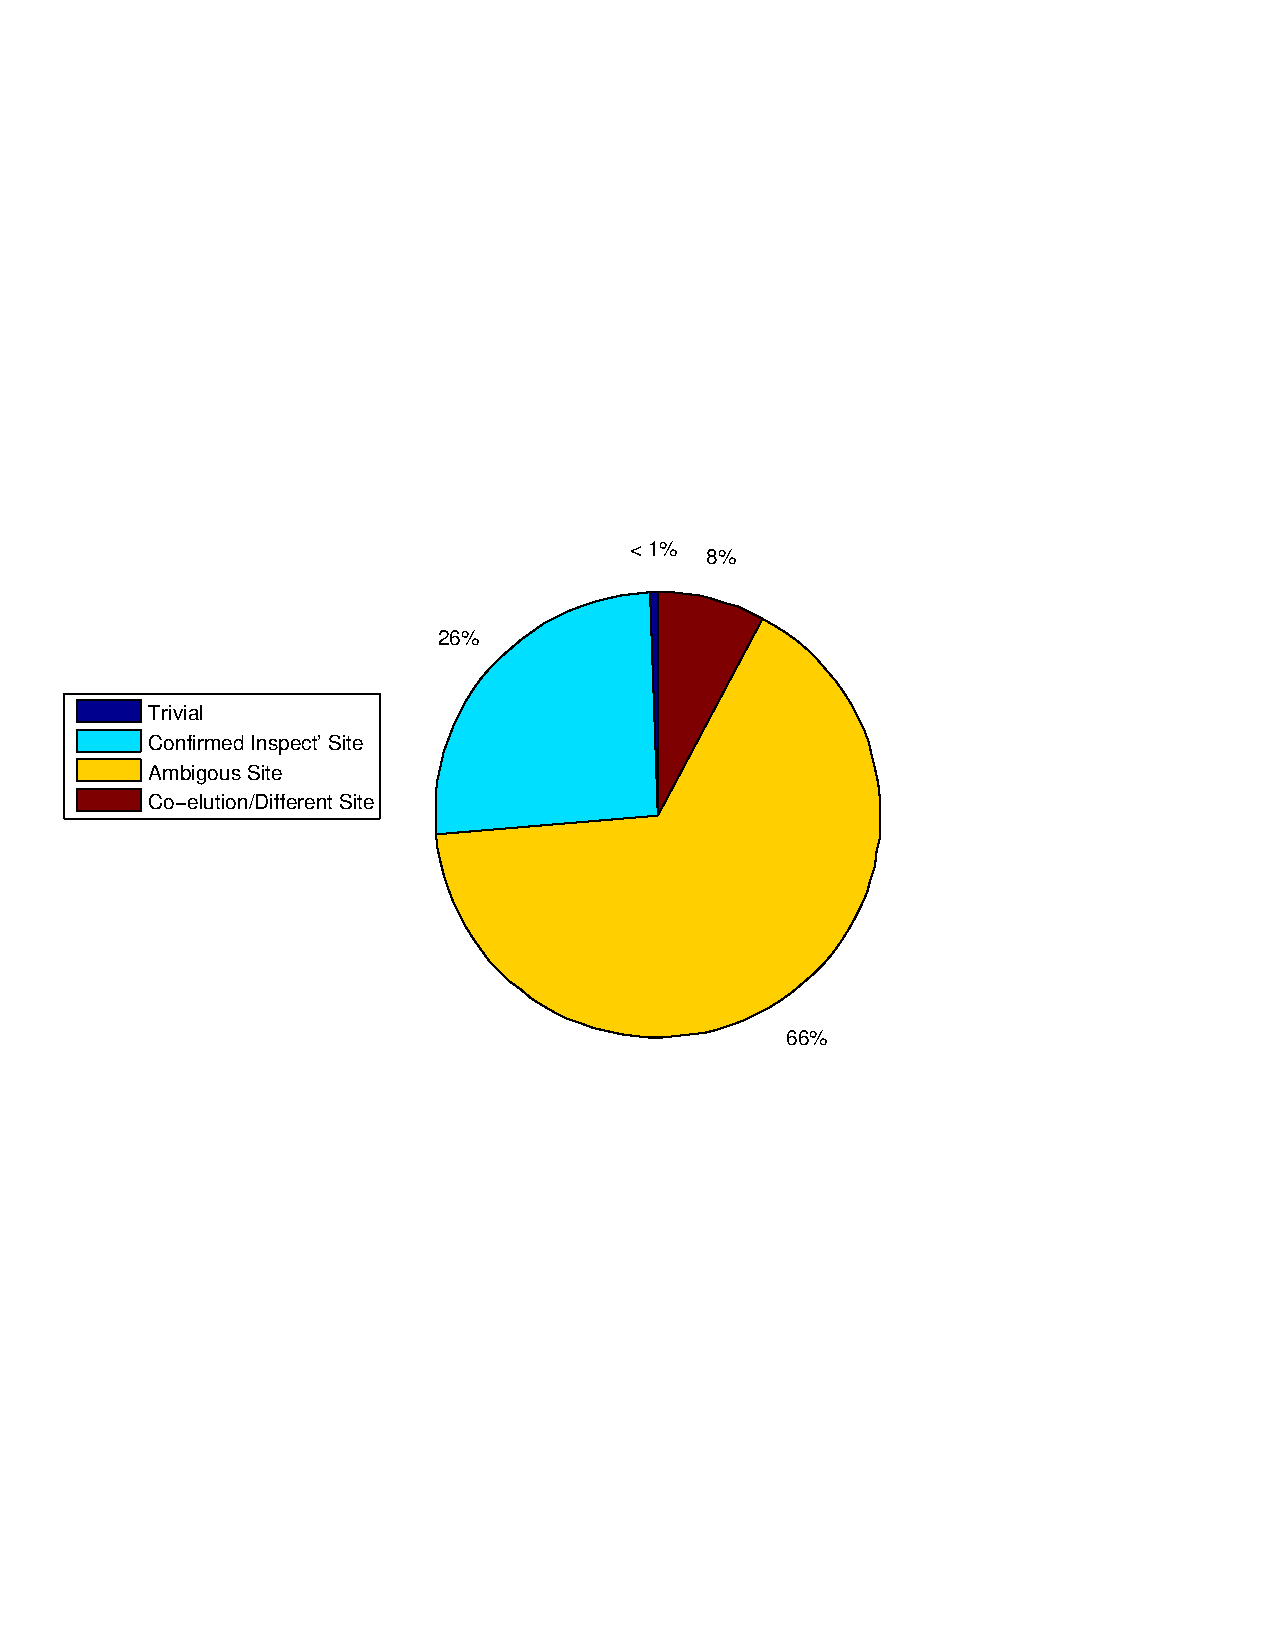
\includegraphics[trim = 0mm 90mm 20mm 90mm,clip,width=0.6\textwidth]{fig/phospho/uniqueIds/piechart_uniq_by_STYDE.pdf}
\caption{Yeast dataset results on unique MS3 -18 peptide identifications: Site assignment results for yeast dataset at $2\%$ FDR.}
\label{fig:yeast_piechart_uniqIds_STYDE}
\end{figure}

\clearpage
\subsubsection{Phosphate Localization Score (PLS)}
\begin{figure}[htbp]
\centering % trim=l b r t
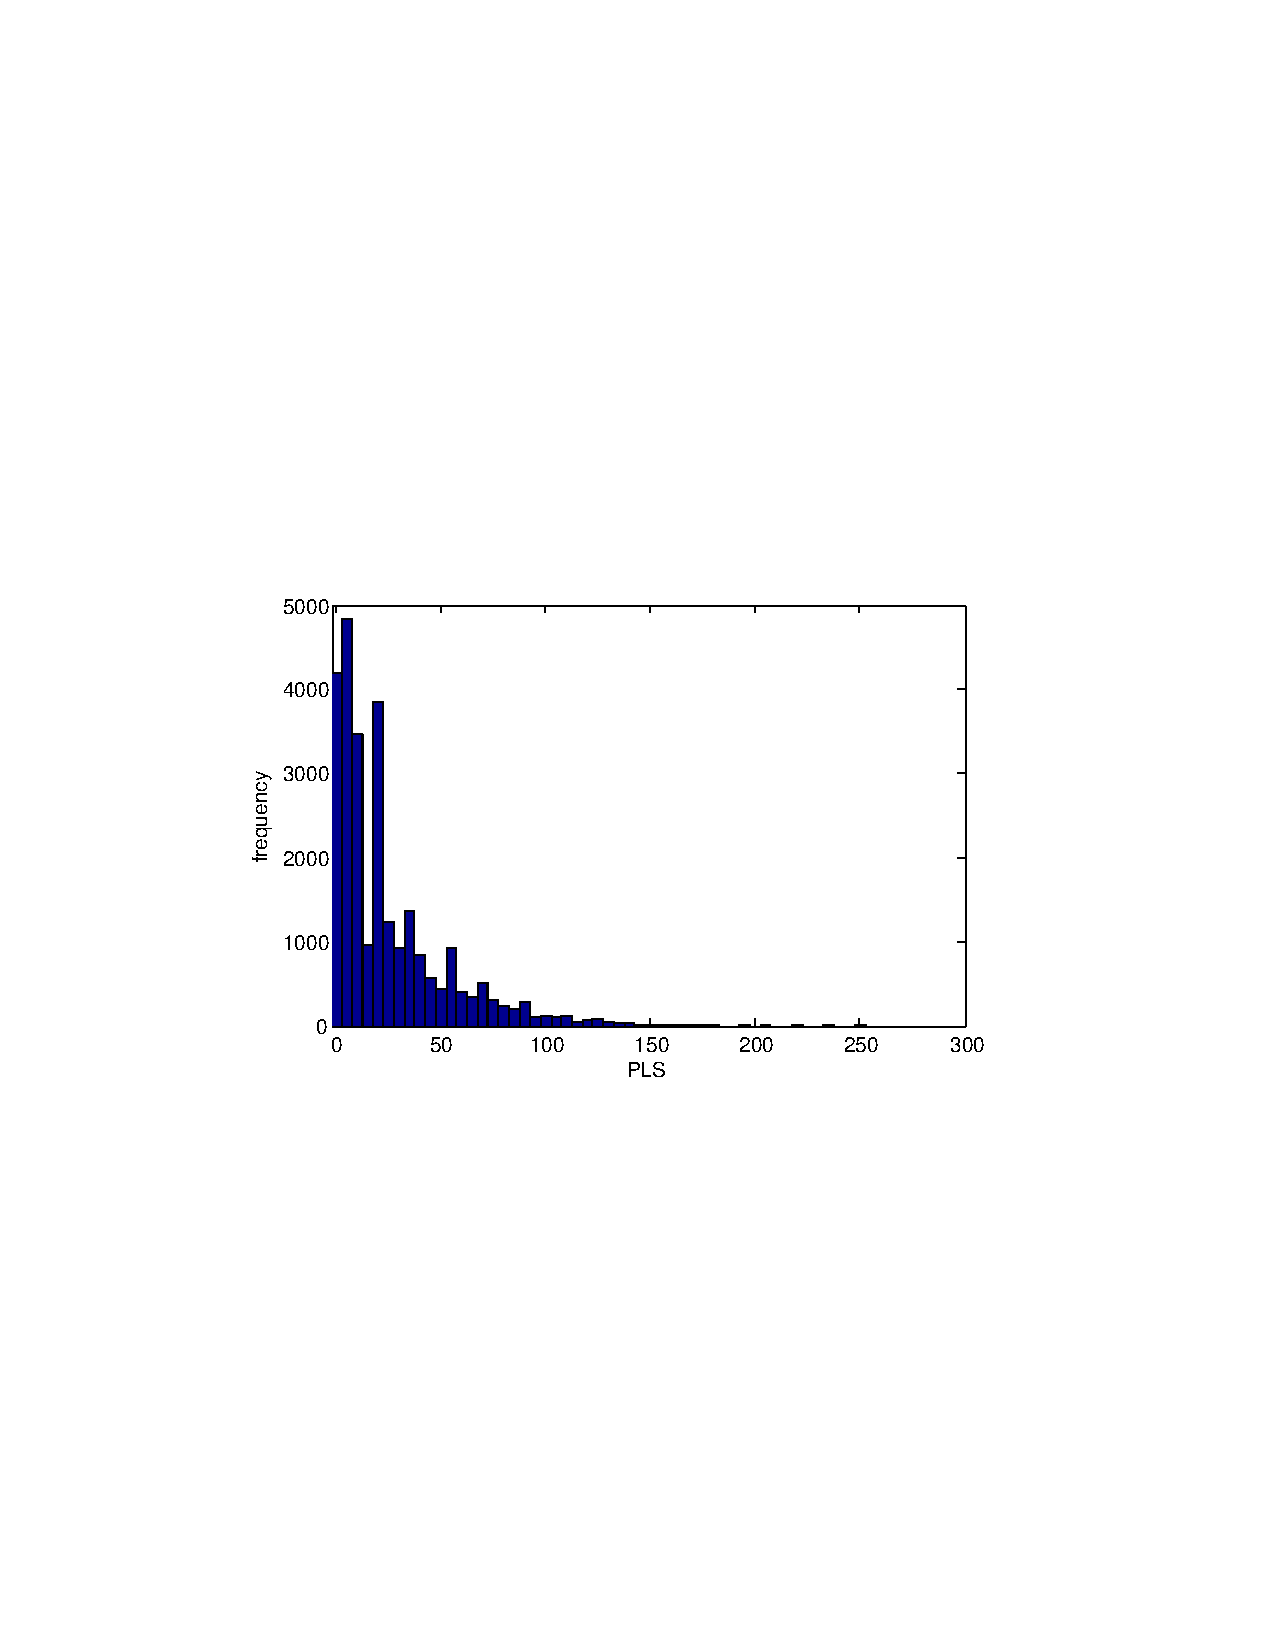
\includegraphics[trim = 0mm 90mm 20mm 90mm,clip,width=0.6\textwidth]{fig/phospho/uniqueIds/PLS_figs/uniqIds_PLS_histogram.pdf}
\caption{Yeast dataset results on unique MS3 -18 peptide identifications: Histogram of PLS. $38\%$ of the PLS scores are $\ge 19$ and $51\%$ are $\ge 13$.}
\label{fig:yeast_pls}
\end{figure}

\begin{figure}[htbp]
\centering % trim=l b r t
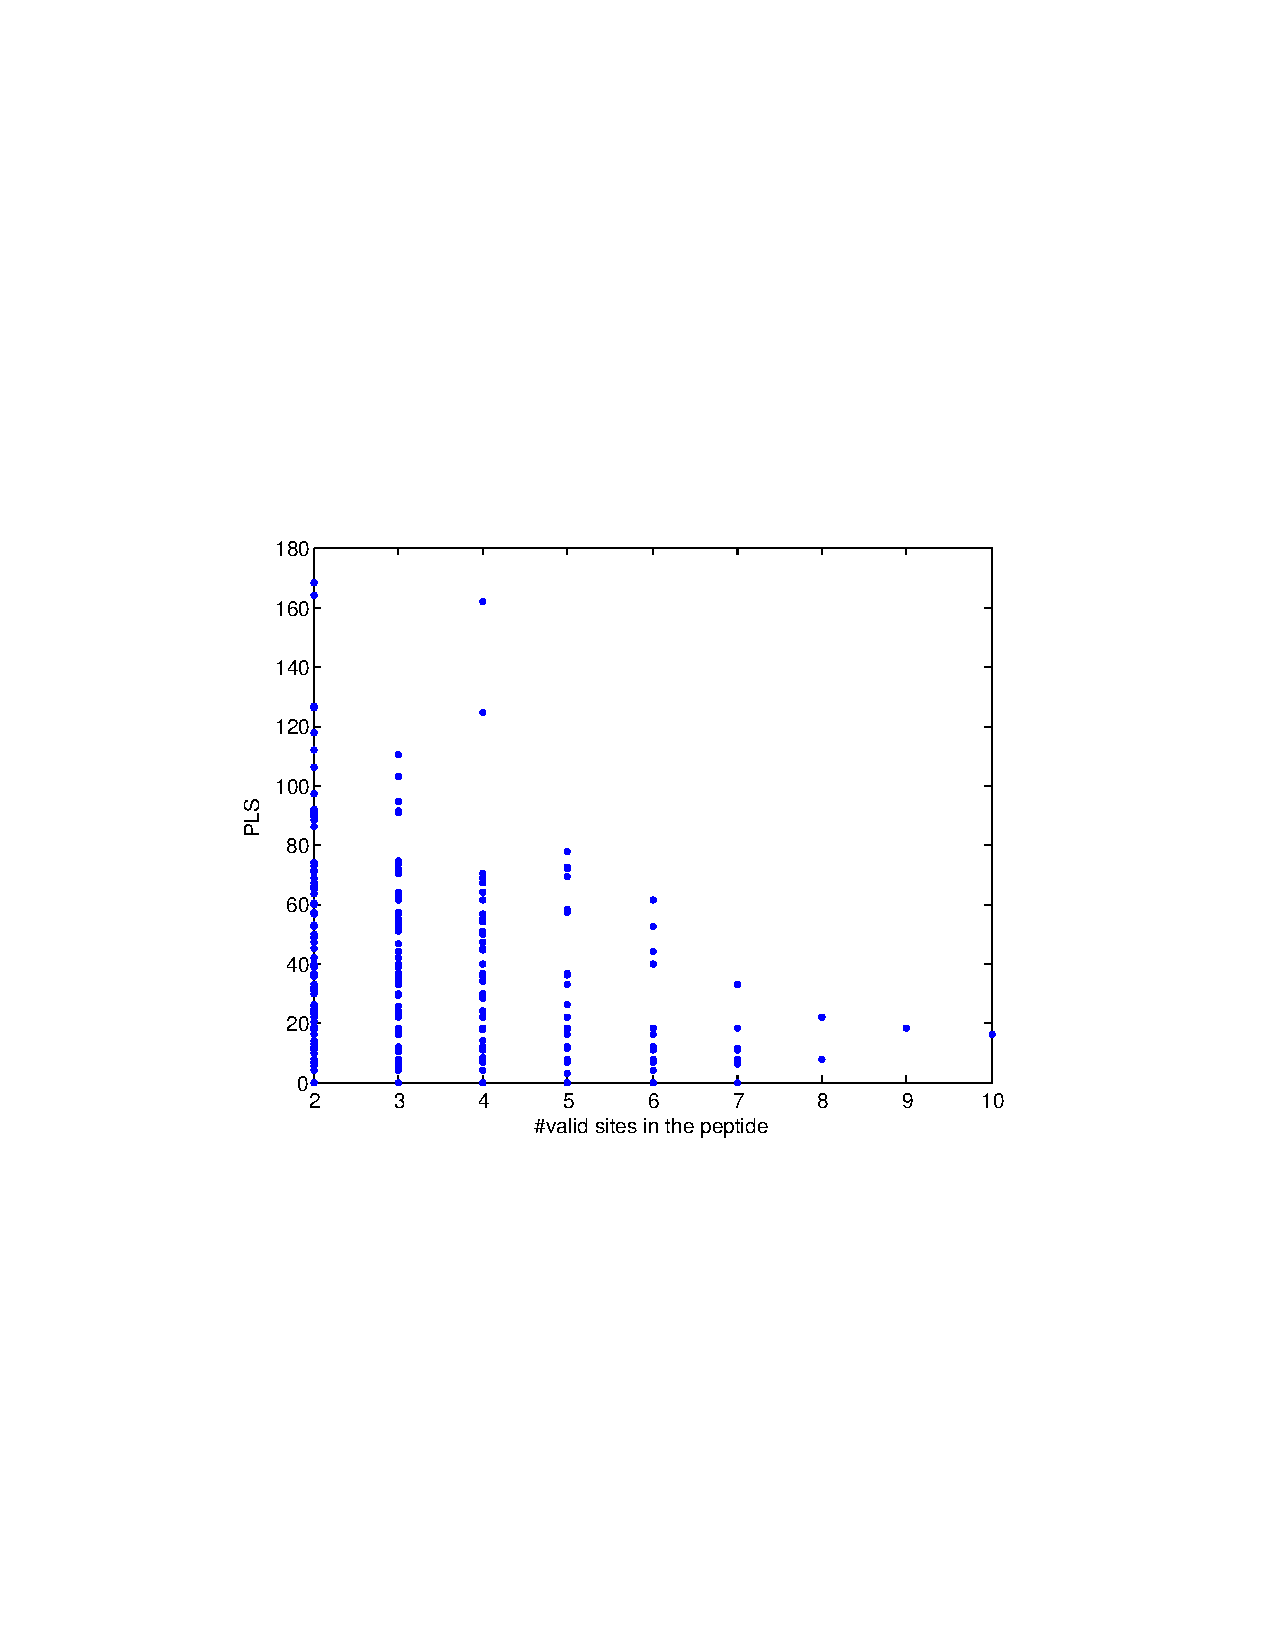
\includegraphics[trim = 0mm 90mm 20mm 90mm,clip,width=0.6\textwidth]{fig/phospho/uniqueIds/PLS_figs/uniqIds_PLS_by_num_valid_sites.pdf}
\caption{Yeast dataset results on unique MS3 -18 peptide identifications: Distribution of PLS by the number of valid sites (S, T, Y) in the peptide.}
\label{fig:yeast_pls}
\end{figure}

\begin{figure}[htbp]
\centering % trim=l b r t
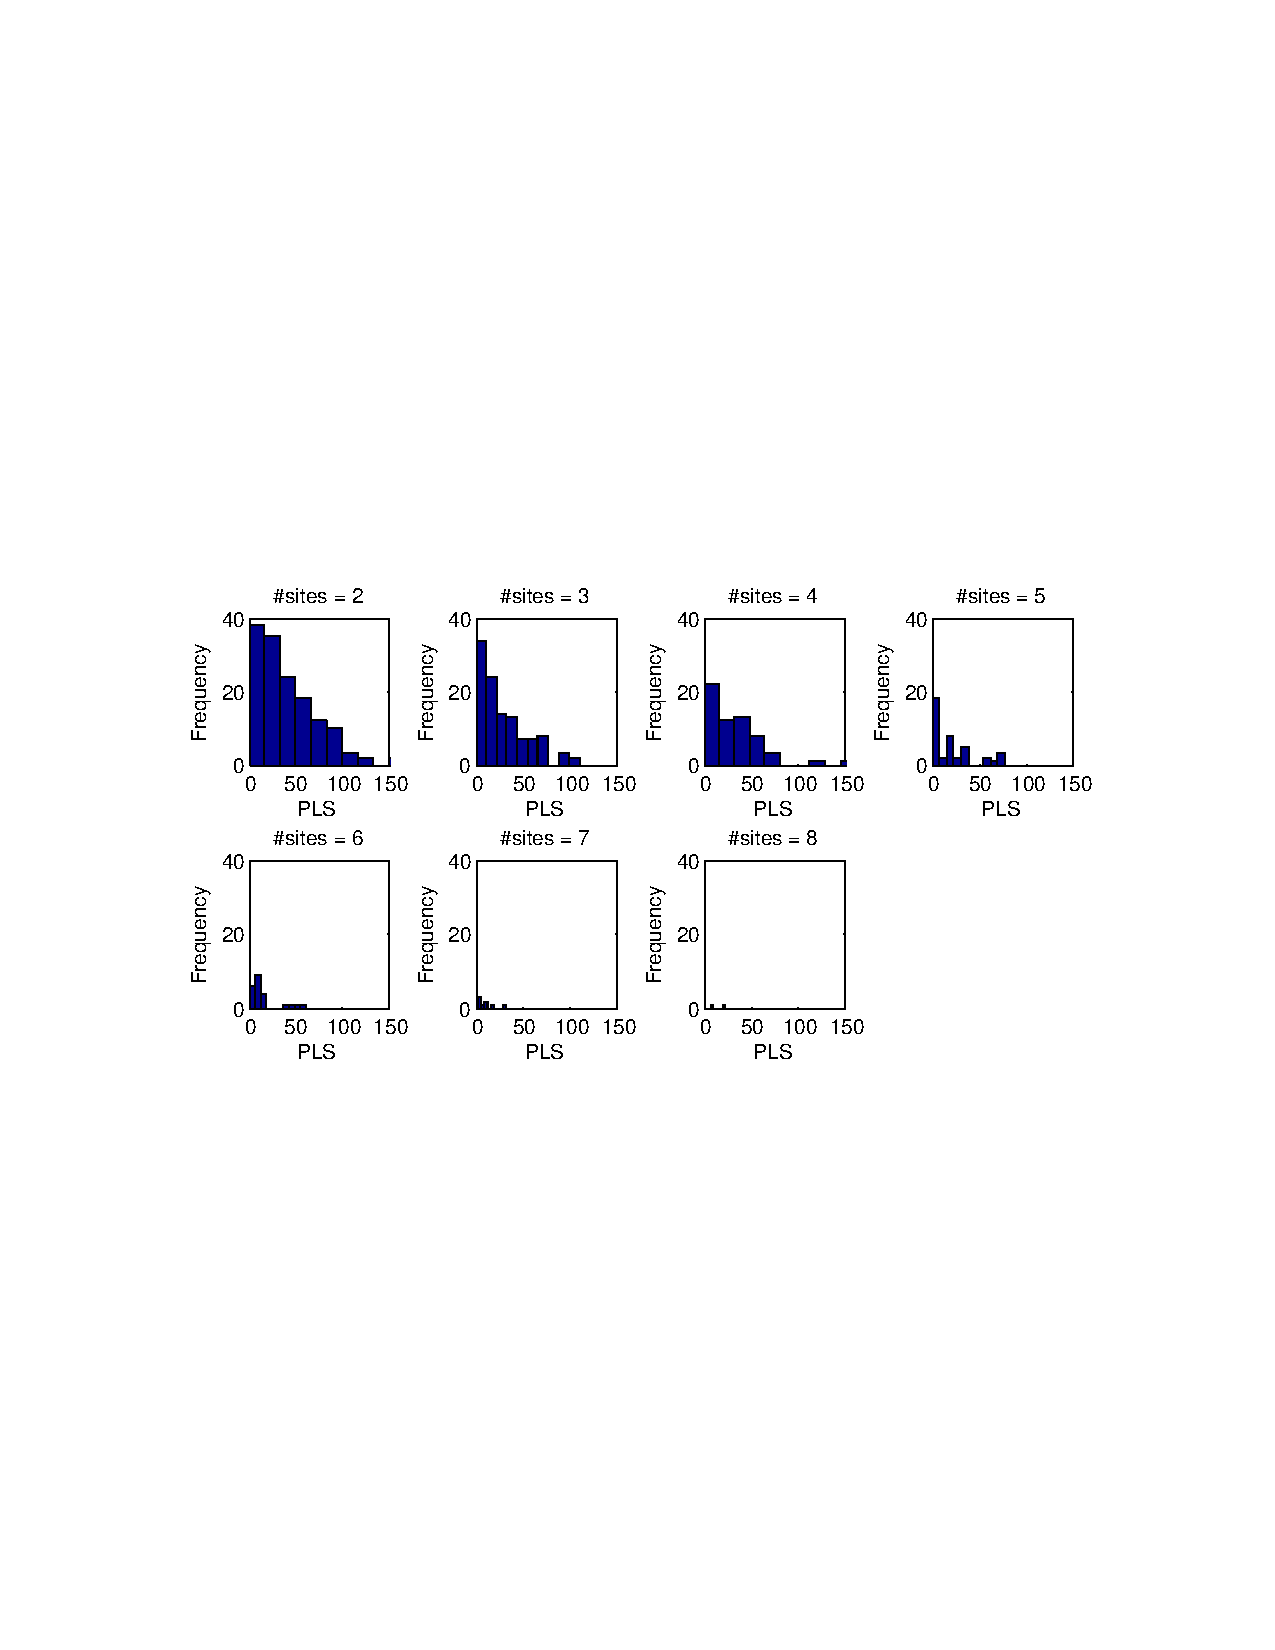
\includegraphics[trim = 0mm 90mm 20mm 90mm,clip,width=\textwidth]{fig/phospho/uniqueIds/PLS_figs/uniqIds_PLS_hist_by_num_valid_sites.pdf}
\caption{Yeast dataset results on unique MS3 -18 peptide identifications: Histogram of PLS by the number of valid sites (S, T, Y) in the peptide.}
\label{fig:yeast_pls}
\end{figure}

\begin{figure}[htbp]
\centering % trim=l b r t
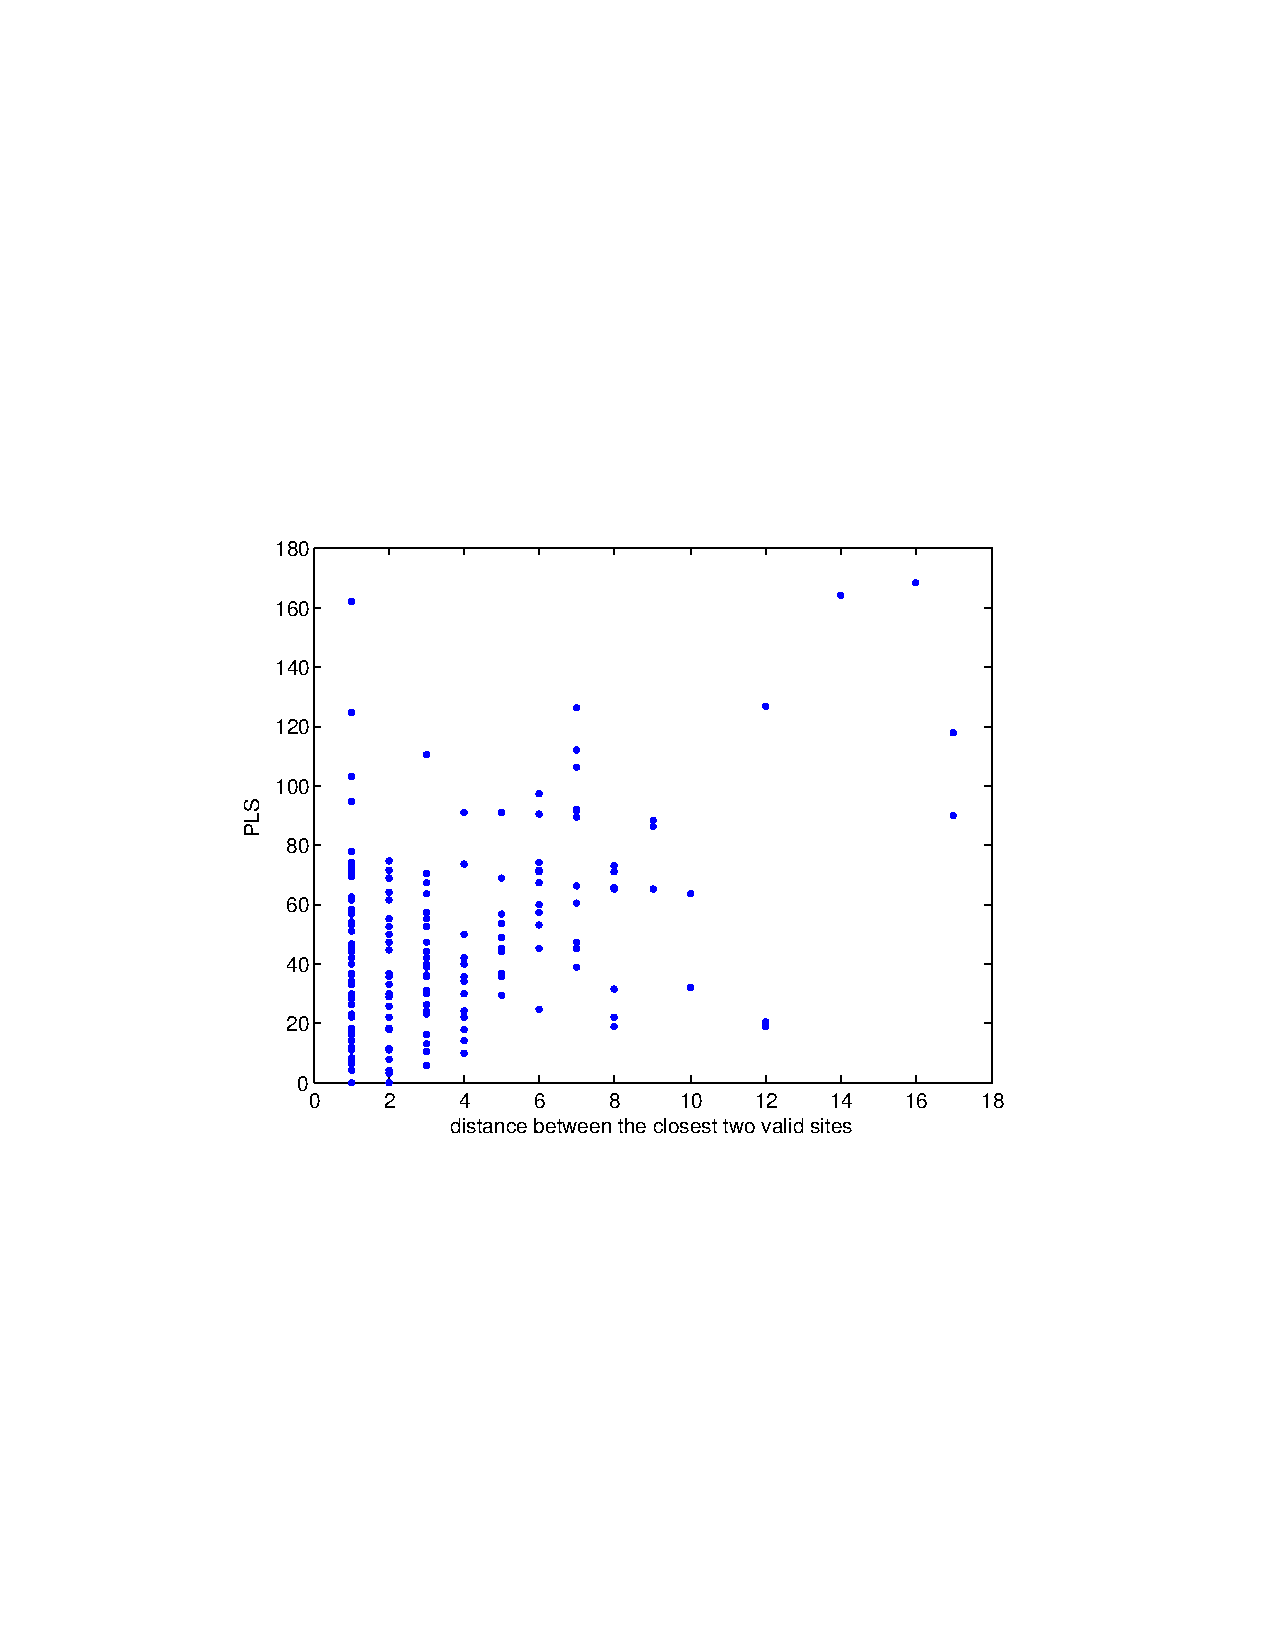
\includegraphics[trim = 0mm 90mm 20mm 90mm,clip,width=0.6\textwidth]{fig/phospho/uniqueIds/PLS_figs/uniqIds_PLS_by_valid_site_distance.pdf}
\caption{Yeast dataset results on unique MS3 -18 peptide identifications: PLS by the distance between the closest two valid sites in the peptide.}
\label{fig:yeast_pls}
\end{figure}


\clearpage
\subsection{Results on all MS3 -18 identifications}

\subsubsection{S,T, and Y are valid sites}

\begin{figure}[htbp]
\centering % trim=l b r t
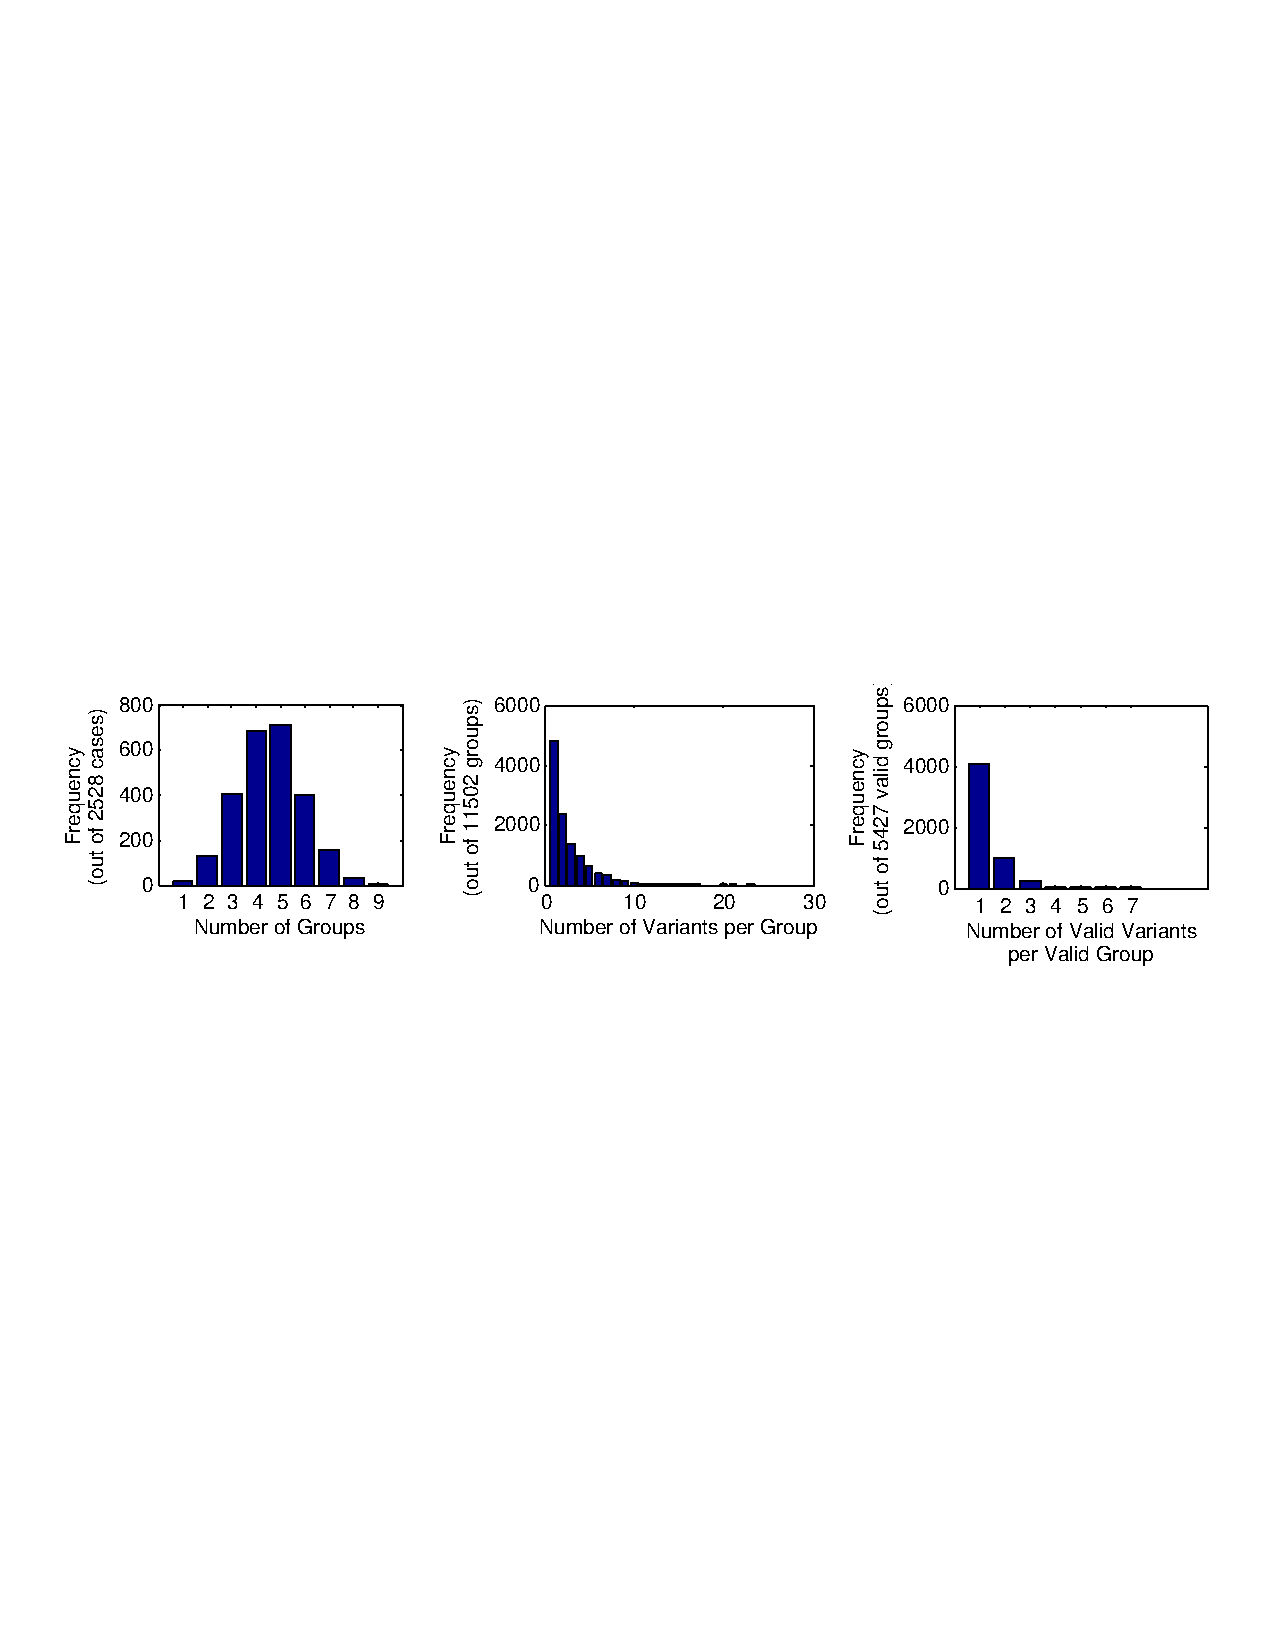
\includegraphics[trim = 2mm 105mm 4mm 105mm,
clip,width=\textwidth]{fig/phospho/allIds/size_dist_all_by_STY.pdf}
\caption{Yeast results on all ids: Distribution of number of variant groups, size of variant groups, and number of valid variants per valid group.}
\label{fig:yeast_sizedist_STY}
\end{figure}


\begin{table}[h]
  \centering
  \caption{Yeast MS3 dataset PTM site assignment FLR results on all peptide identifications. At cosine score cutoff = $0.4$, $277$ cases rejected, $2251$ cases accepted. S, T and Y are considered as valid sites.}\label{tbl:YeastFLR_all_STY}
\begin{tabular}{|c|l|l|l|l|l|}
\hline
Estimated Abundance & \multirow{2}{*}{FDR} & \multicolumn{4}{|c|}{\#Cases with k groups identified }\\
of Variant Group & & $k\ge 1$ & $k=1$ & $k=2$ & $k=3$\\
\hline
$\ge	60	\%$ &	0.05	\% &	90.3	\% &	90.3	\% &	0.0	\% &	0.0	\\
$\ge	55	\%$ &	0.06	\% &	91.5	\% &	91.5	\% &	0.0	\% &	0.0	\\
$\ge	50	\%$ &	0.06	\% &	92.5	\% &	92.5	\% &	0.0	\% &	0.0	\\
$\ge	45	\%$ &	0.06	\% &	93.4	\% &	93.2	\% &	0.2	\% &	0.0	\\
$\ge	40	\%$ &	0.07	\% &	93.8	\% &	93.2	\% &	0.6	\% &	0.0	\\
$\ge	35	\%$ &	0.08	\% &	94.2	\% &	93.3	\% &	0.9	\% &	0.0	\\
$\ge	30	\%$ &	0.09	\% &	94.4	\% &	92.9	\% &	1.5	\% &	0.0	\\
$\ge	25	\%$ &	0.11	\% &	94.8	\% &	92.4	\% &	2.4	\% &	0.0	\\
$\ge	20	\%$ &	0.14	\% &	94.9	\% &	91.4	\% &	3.3	\% &	0.1	\\
$\ge	15	\%$ &	0.17	\% &	95.4	\% &	90.3	\% &	4.9	\% &	0.1	\\
%$\ge	10	\%$ &	0.23	\% &	95.8	\% &	87.9	\% &	7.5	\% &	0.4	\\
%$\ge	5	\%$ &	0.30	\% &	96.5	\% &	83.0	\% &	12.9	\% &	0.6	\\

\hline
\end{tabular}
\end{table}

\begin{figure}[htbp]
\centering % trim=l b r t
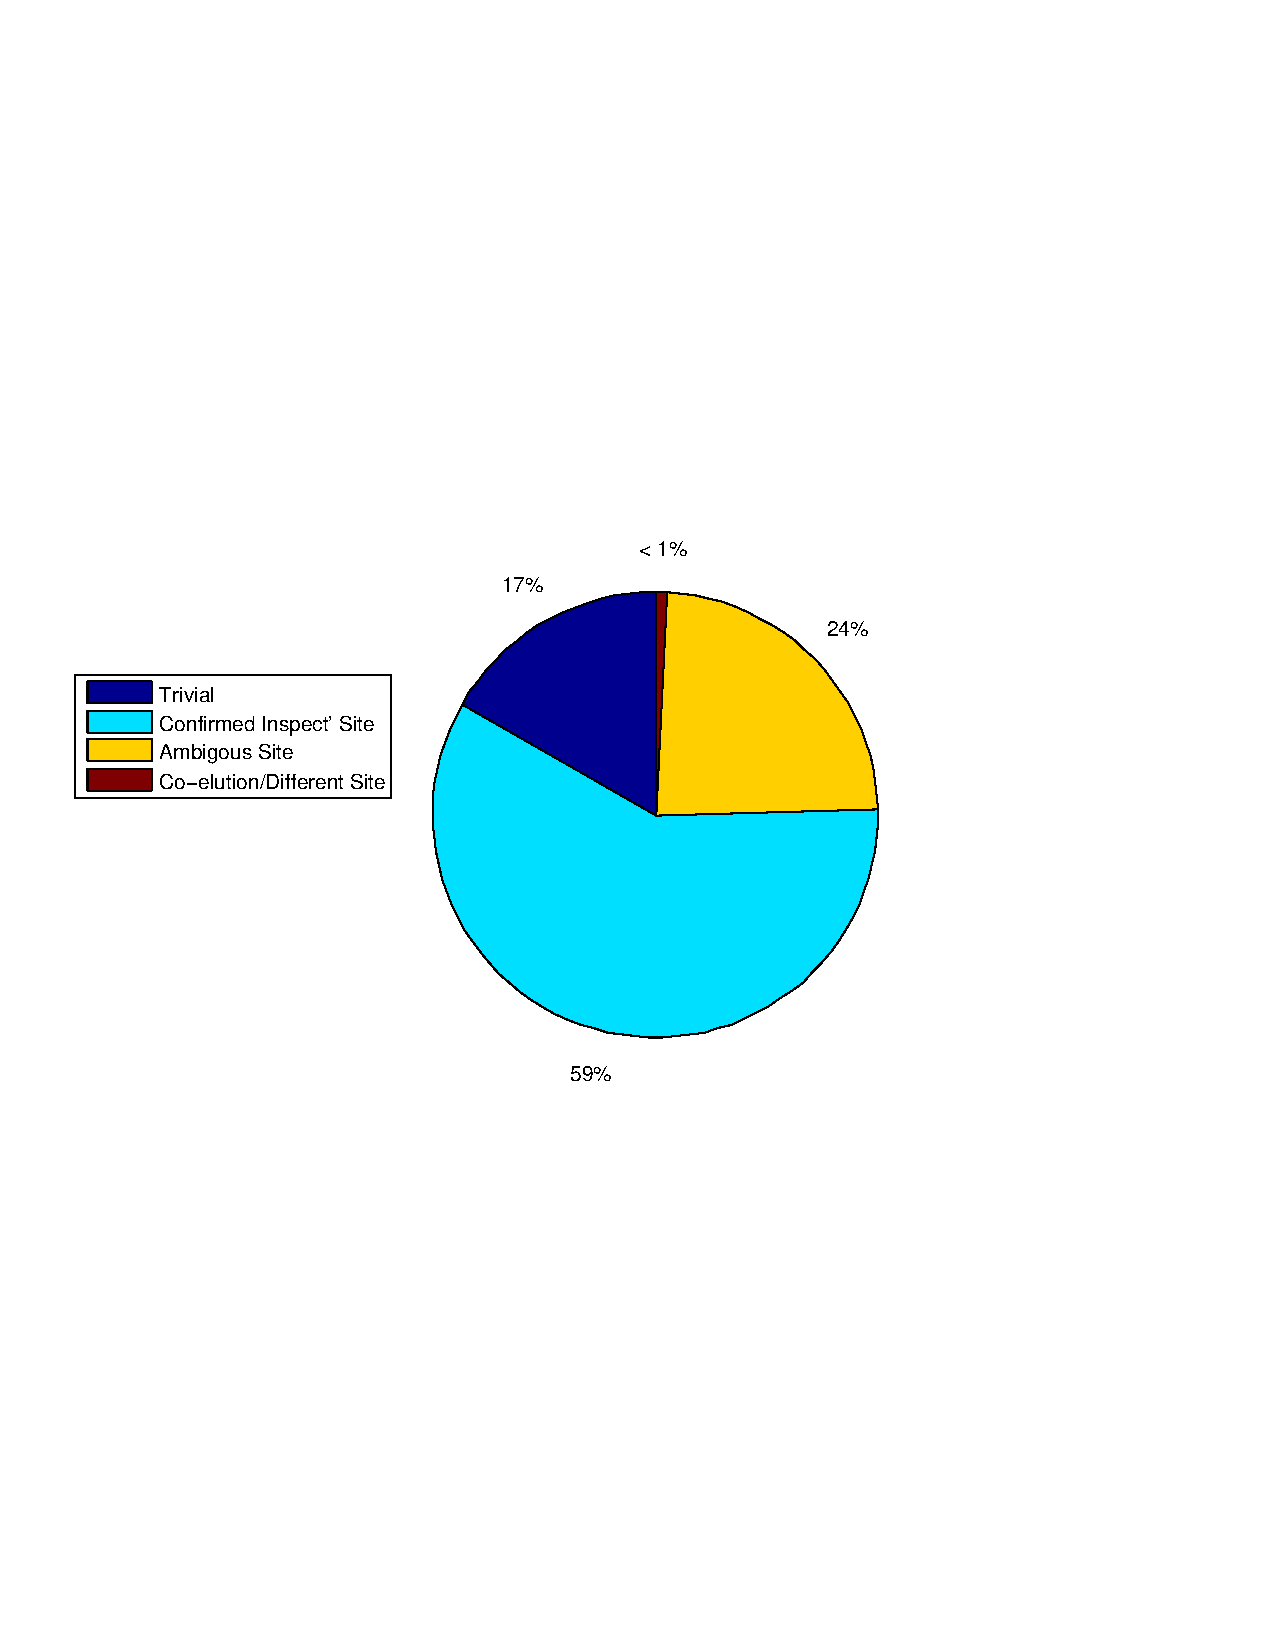
\includegraphics[trim = 0mm 90mm 20mm 90mm,clip,width=0.6\textwidth]{fig/phospho/allIds/piechart_all_by_STY.pdf}
\caption{Yeast dataset results on unique MS3 -18 peptide identifications: Site assignment results for yeast dataset at $3\%$ FDR.}
\label{fig:yeast_piechart_uniqIds_STY}
\end{figure}

\clearpage
\subsubsection{S,T,Y,D, and E are valid sites}
\begin{figure}[htbp]
\centering % trim=l b r t
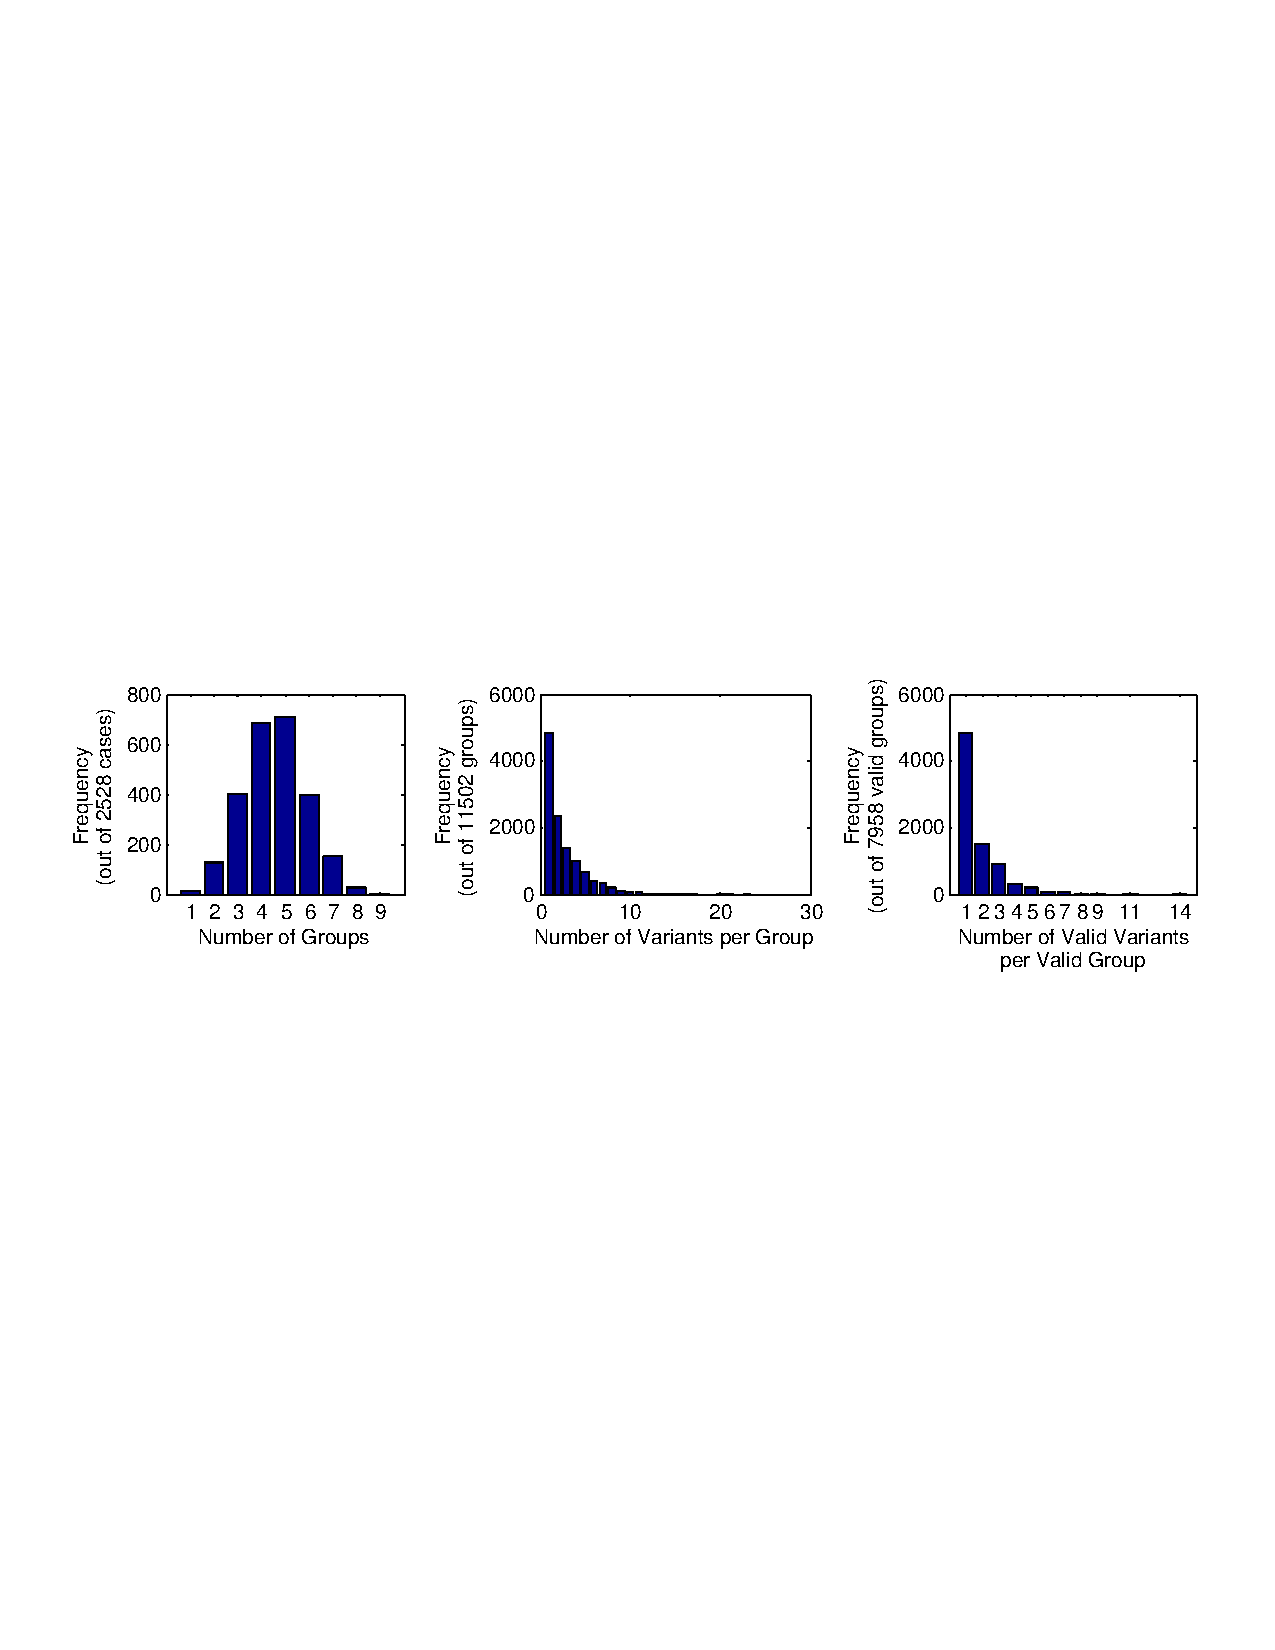
\includegraphics[trim = 2mm 105mm 4mm 105mm,
clip,width=\textwidth]{fig/phospho/allIds/size_dist_all_by_STYDE.pdf}
\caption{Yeast results on all ids: Distribution of number of variant groups, size of variant groups, and number of valid variants per valid group.}
\label{fig:yeast_sizedist_STYDE}
\end{figure}

\begin{table}[h]
  \centering
  \caption{Yeast MS3 dataset PTM site assignment FLR results on all peptide identifications. At cosine score cutoff = $0.4$, $277$ cases rejected, $2251$ cases accepted. S, T, Y, D and E are considered as valid sites.}\label{tbl:YeastFLR_all_STYDE}
\begin{tabular}{|c|l|l|l|l|l|l|}
\hline
Estimated Abundance & \multirow{2}{*}{FDR} & \multicolumn{5}{|c|}{\#Cases with k groups identified }\\
of Variant Group & & $k\ge 1$ & $k=1$ & $k=2$ & $k=3$  & $k=4$\\
\hline
$\ge	60	\%$ &	0.05	\% &	90.8	\% &	90.8	\% &	0.0	\% &	0.0	\% &	0.0	\\
$\ge	55	\%$ &	0.06	\% &	92.0	\% &	92.0	\% &	0.0	\% &	0.0	\% &	0.0	\\
$\ge	50	\%$ &	0.06	\% &	93.2	\% &	92.9	\% &	0.2	\% &	0.0	\% &	0.0	\\
$\ge	45	\%$ &	0.06	\% &	94.0	\% &	93.4	\% &	0.5	\% &	0.0	\% &	0.0	\\
$\ge	40	\%$ &	0.06	\% &	94.6	\% &	93.3	\% &	1.2	\% &	0.0	\% &	0.0	\\
$\ge	35	\%$ &	0.07	\% &	95.1	\% &	93.2	\% &	1.9	\% &	0.0	\% &	0.0	\\
$\ge	30	\%$ &	0.07	\% &	95.6	\% &	92.8	\% &	2.8	\% &	0.0	\% &	0.0	\\
$\ge	25	\%$ &	0.08	\% &	96.5	\% &	91.9	\% &	4.5	\% &	0.1	\% &	0.0	\\
$\ge	20	\%$ &	0.08	\% &	97.5	\% &	90.6	\% &	6.6	\% &	0.3	\% &	0.0	\\
$\ge	15	\%$ &	0.10	\% &	98.5	\% &	88.1	\% &	9.6	\% &	0.8	\% &	0.0	\\
%$\ge	10	\%$ &	0.12	\% &	99.2	\% &	82.7	\% &	15.0	\% &	1.4	\% &	0.1	\\
%$\ge	5	\%$ &	0.15	\% &	99.6	\% &	74.3	\% &	21.6	\% &	3.4	\% &	0.2	\\
\hline
\end{tabular}
\end{table}

\begin{figure}[htbp]
\centering % trim=l b r t
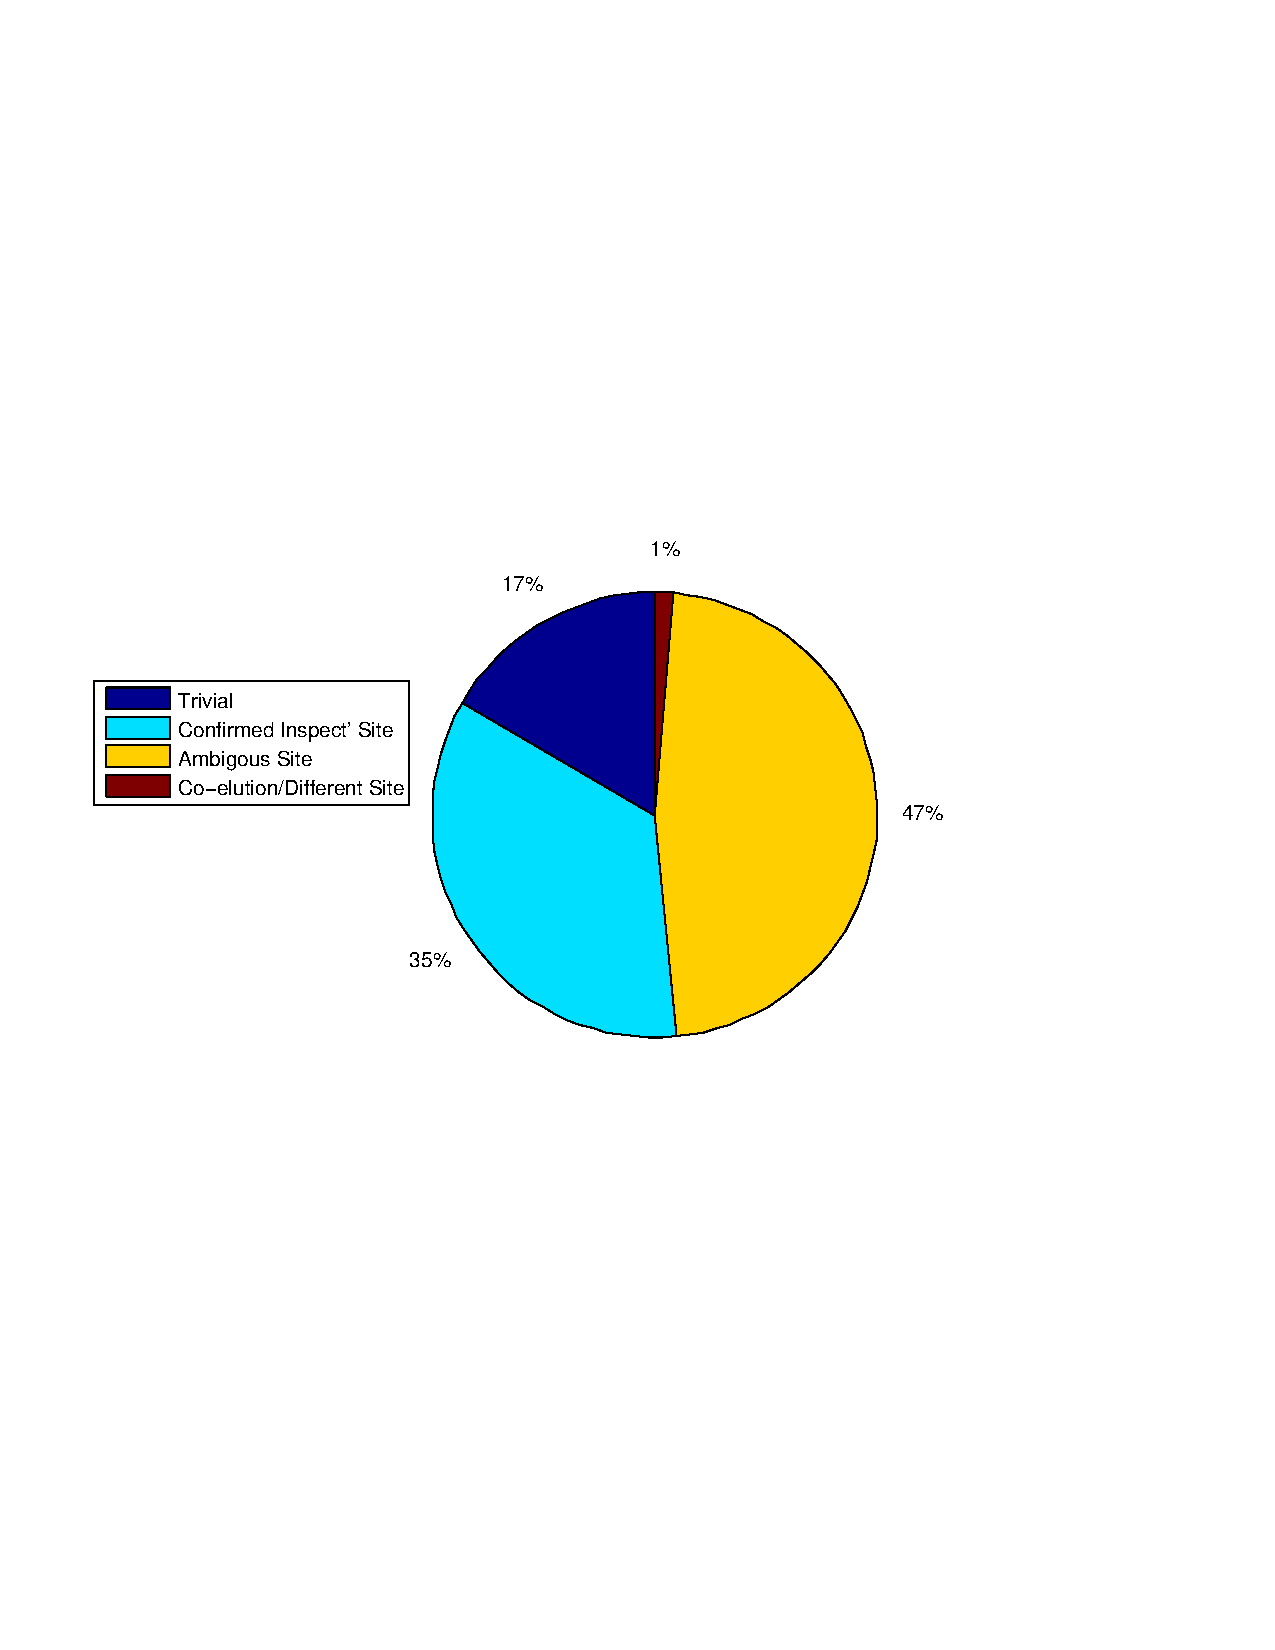
\includegraphics[trim = 0mm 90mm 20mm 90mm,clip,width=0.6\textwidth]{fig/phospho/allIds/piechart_all_by_STYDE.pdf}
\caption{Yeast dataset results on unique MS3 -18 peptide identifications: Site assignment results for yeast dataset at $2\%$ FDR.}
\label{fig:yeast_piechart_uniqIds_STYDE}
\end{figure}

\clearpage
\subsubsection{Phosphate Localization Score (PLS)}
\begin{figure}[htbp]
\centering % trim=l b r t
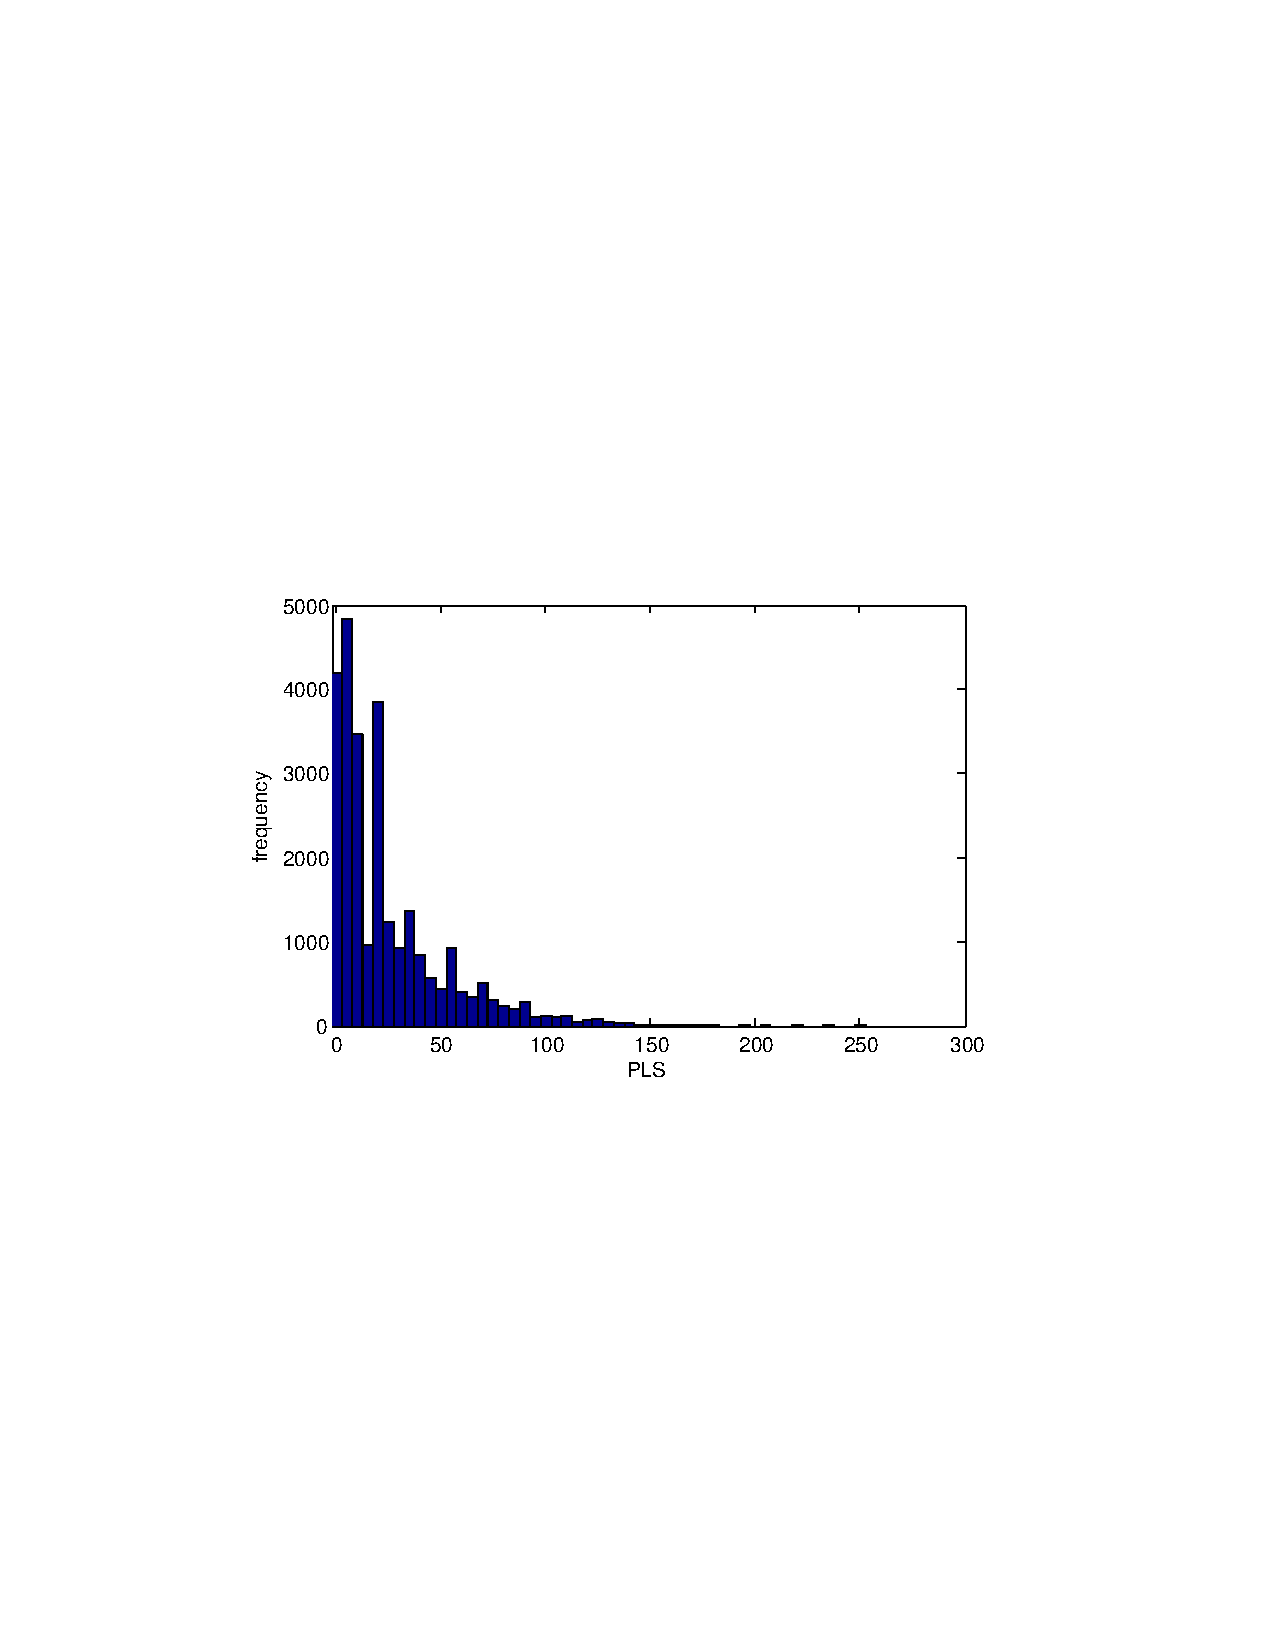
\includegraphics[trim = 0mm 90mm 20mm 90mm,clip,width=0.6\textwidth]{fig/phospho/allIds/PLS_figs/allIds_PLS_histogram.pdf}
\caption{Yeast dataset results on all MS3 -18 peptide identifications: Histogram of PLS. $38\%$ of the PLS scores are $\ge 19$ and $51\%$ are $\ge 13$.}
\label{fig:yeast_pls}
\end{figure}

\begin{figure}[htbp]
\centering % trim=l b r t
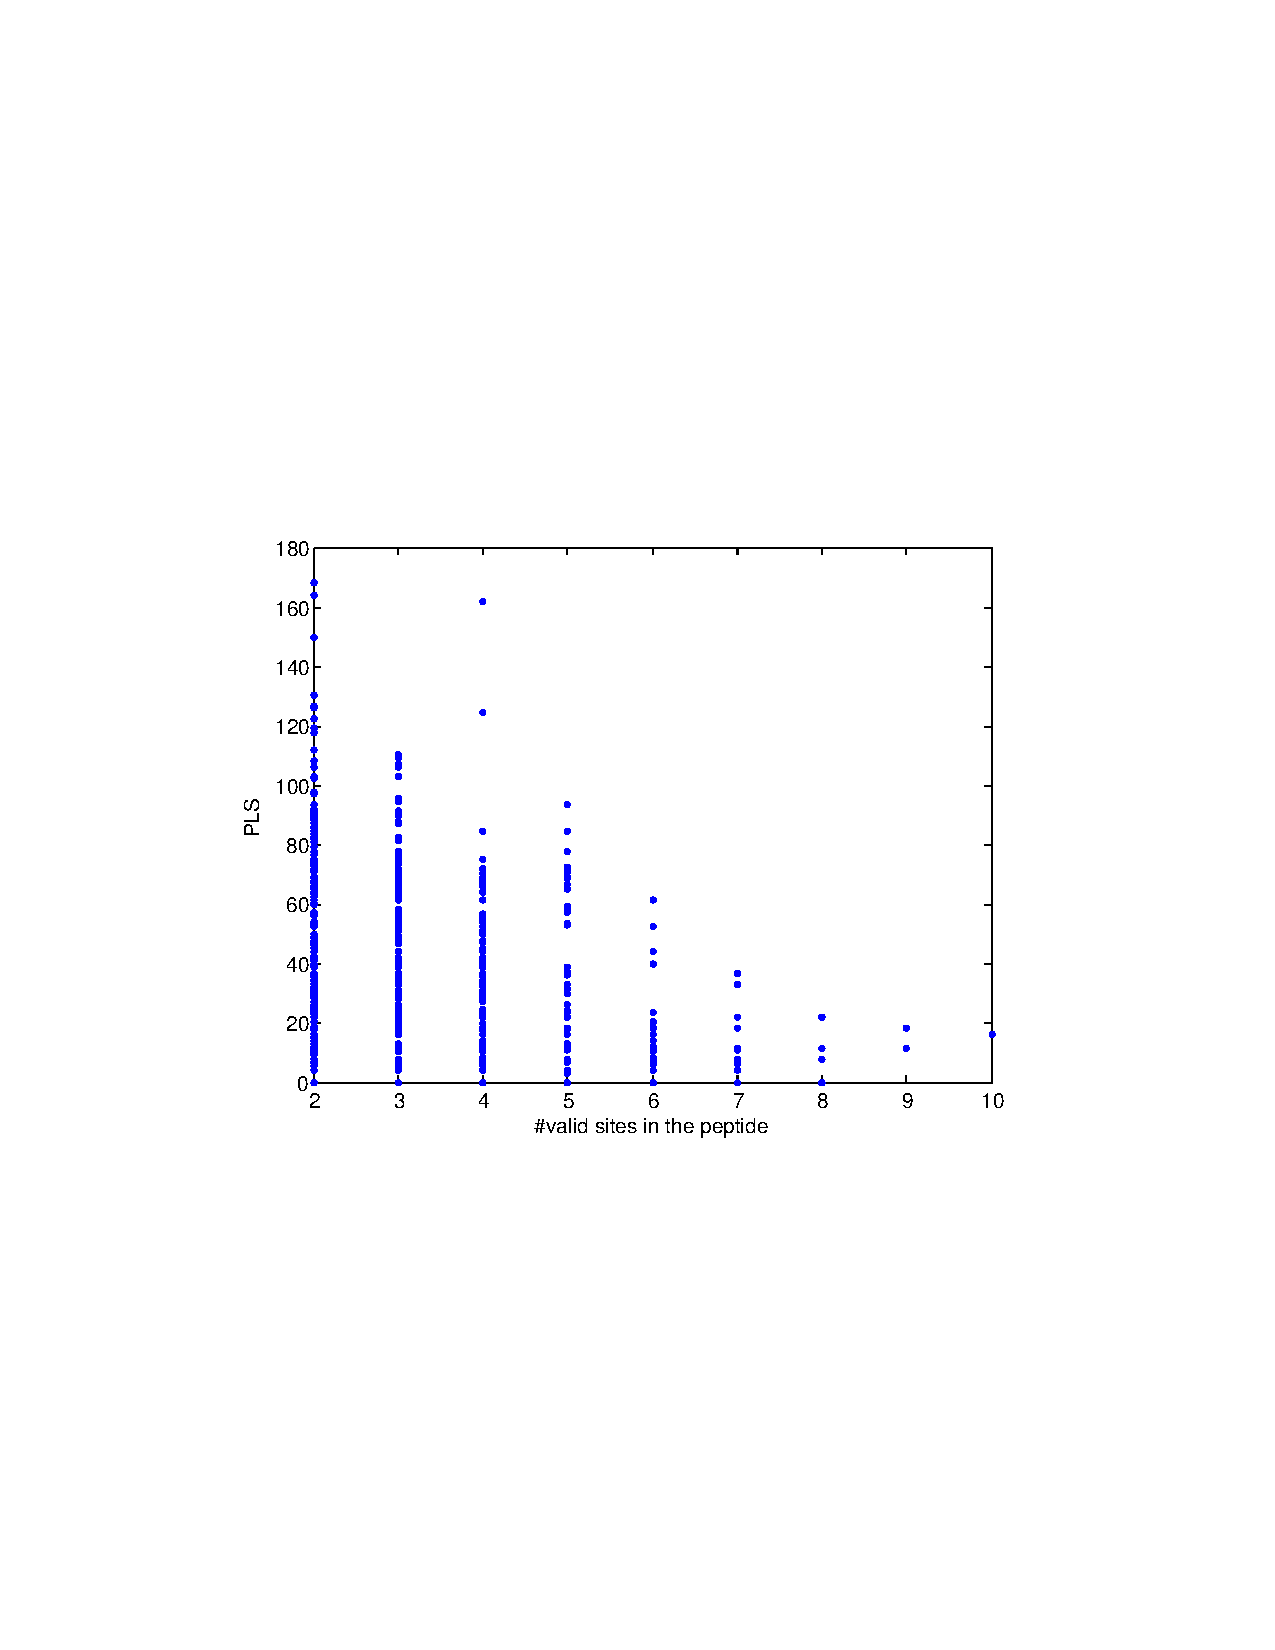
\includegraphics[trim = 0mm 90mm 20mm 90mm,clip,width=0.6\textwidth]{fig/phospho/allIds/PLS_figs/allIds_PLS_by_num_valid_sites.pdf}
\caption{Yeast dataset results on all MS3 -18 peptide identifications: Distribution of PLS by the number of valid sites (S, T, Y) in the peptide.}
\label{fig:yeast_pls}
\end{figure}

\begin{figure}[htbp]
\centering % trim=l b r t
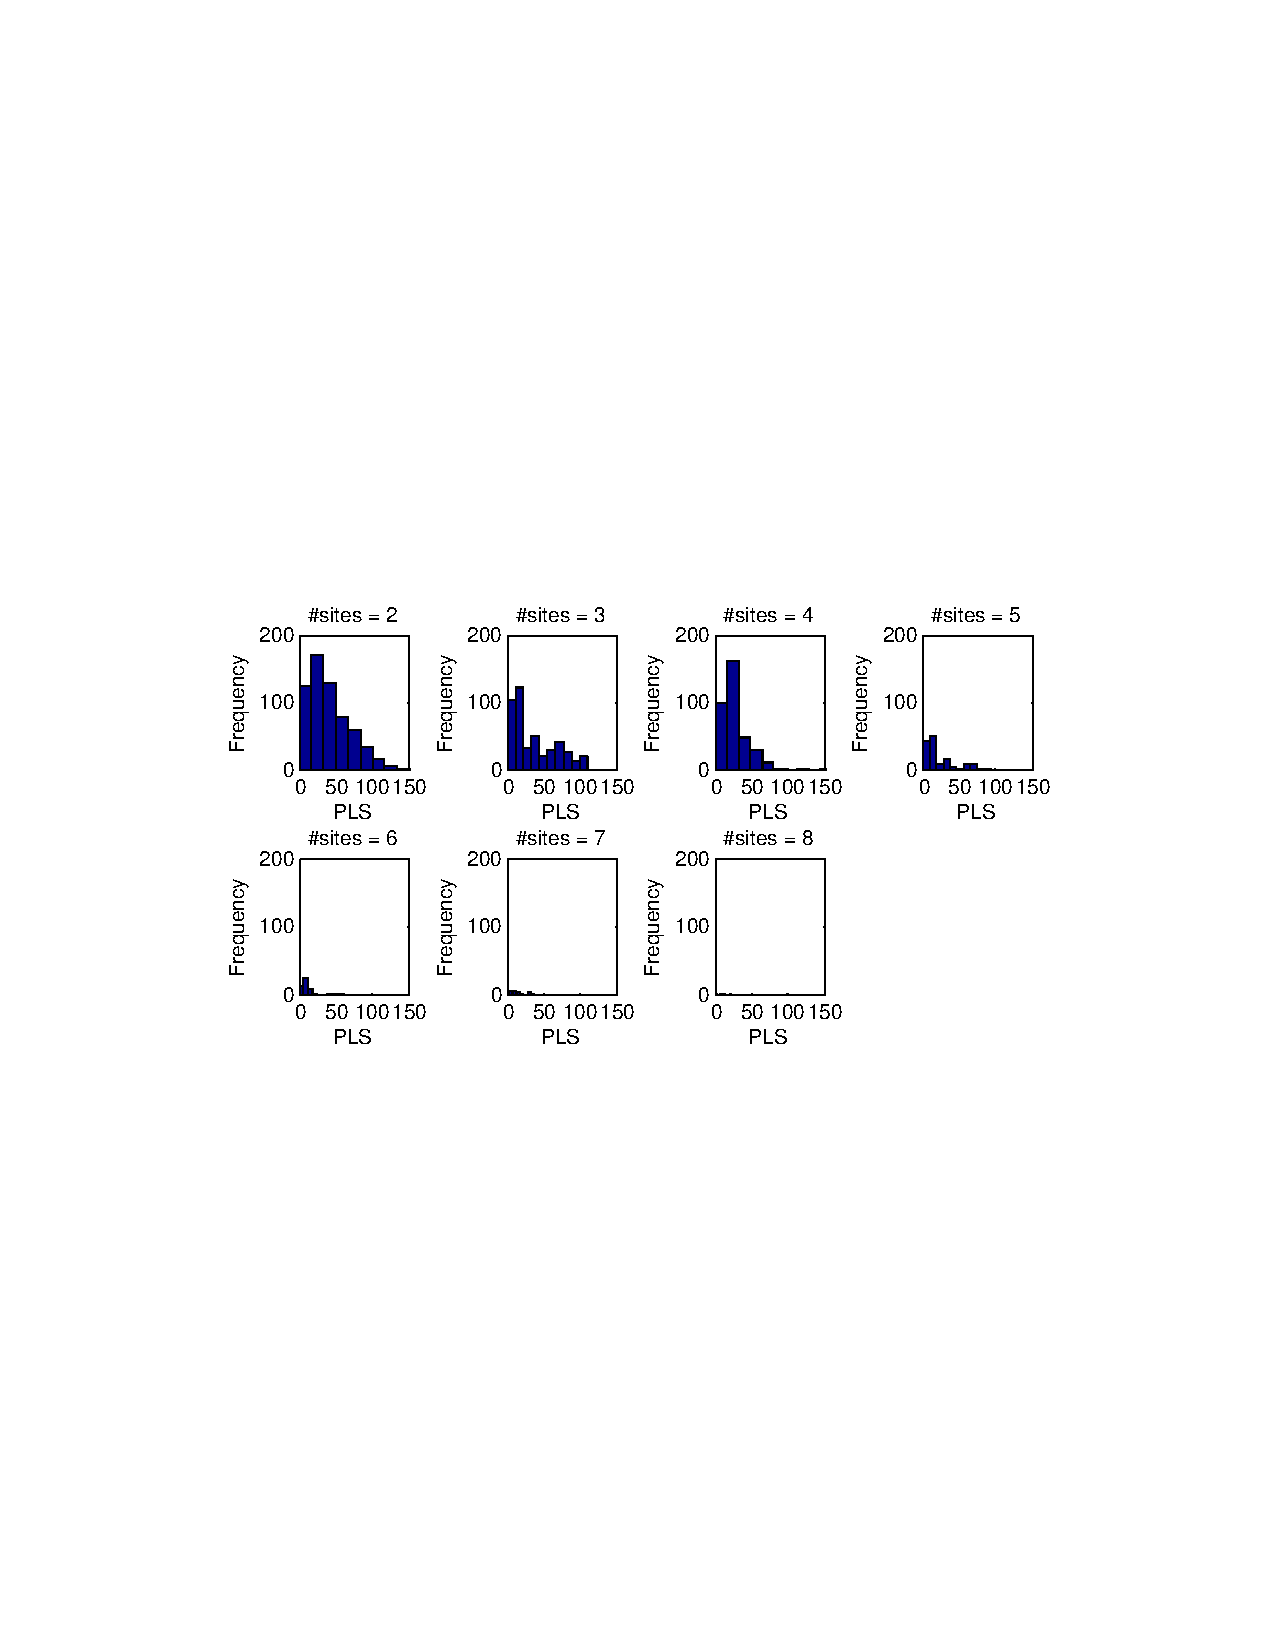
\includegraphics[trim = 0mm 90mm 20mm 90mm,clip,width=\textwidth]{fig/phospho/allIds/PLS_figs/allIds_PLS_hist_by_num_valid_sites.pdf}
\caption{Yeast dataset results on all MS3 -18 peptide identifications: Histogram of PLS by the number of valid sites (S, T, Y) in the peptide.}
\label{fig:yeast_pls}
\end{figure}

\begin{figure}[htbp]
\centering % trim=l b r t
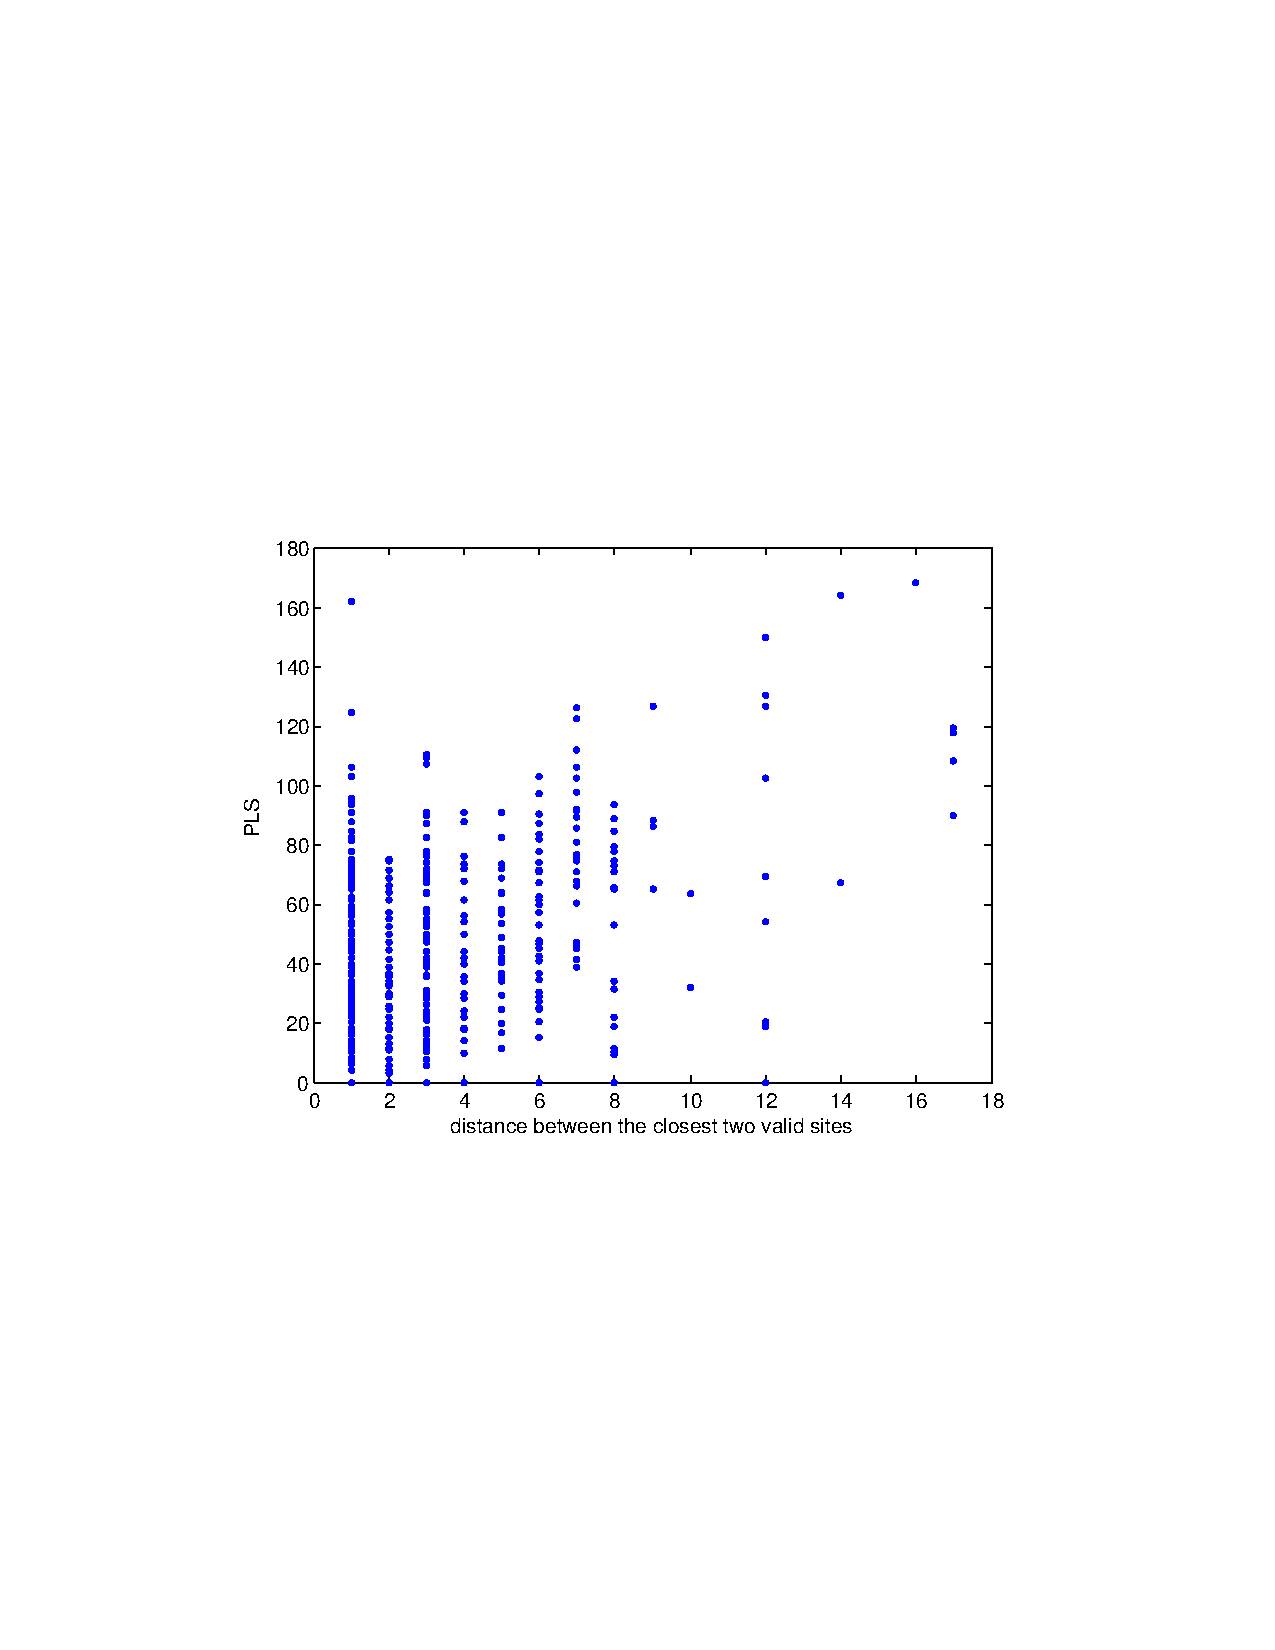
\includegraphics[trim = 0mm 90mm 20mm 90mm,clip,width=0.6\textwidth]{fig/phospho/allIds/PLS_figs/allIds_PLS_by_valid_site_distance.pdf}
\caption{Yeast dataset results on all MS3 -18 peptide identifications: PLS by the distance between the closest two valid sites in the peptide.}
\label{fig:yeast_pls}
\end{figure}

